\documentclass[a4paper,english,11pt,]{scrartcl}
\usepackage{mystyle}

\title{Statische Modellen \& Data-analyse}
\subtitle{Homework 2}
\author{Andreas Put \and Li Quan}
%\subject{Verslag}
\date{May 23, 2011}
\bibliographystyle{abbrv}

\begin{document}
\maketitle

%% inleiding + beschrijving dataset (variabelen + achtergrond)
%% pca+pcr+pls, lineair model, variable selectie (forward,backward stepwise regression) -> price berekenen (zonder en met boxcox transformatie)
%% anova, pairwise tests
%% conclusie dataset
\section{Introduction}
We analyze the \emph{autos} dataset of the UCI Machine Learning Repository which can be found at \url{http://archive.ics.uci.edu/ml/machine-learning-databases/autos/}.
We first give a short overview of the dataset and than discuss our analysis of the dataset.

\section{Description dataset}
\input{datasetdescription.tex}

\section{Dataset exploration and preprocessing}

The dataset contains $p=26$ attributes, and $n=206$ observations. It also contains some instances with missing attribute values, especially for normalized losses. Because we have a large amount of data ($n>5p$), we chose to simply omit observations with any missing attribute values. If we do this, we still have plenty of data to use---more specifically $n=159$ observations---which is why we chose this method instead of replacing them with for instance variable means or interpolations \cite{missingvalues}.

We have an \emph{exploratory observational} dataset. A tool such as ggobi\footnote{\url{http://www.ggobi.org/}} allows us to visualize the data in different ways to get familiar with the dataset. This way, we interactively searched for extreme outliers and screened explanatory variables.

We found out that the variable `engine-location' only had 3 instances of `rear' (0 after removing instances with missing values) which is why we can easily discard this variable. Furthermore, as we have such a highly dimensional dataset, for our analysis we will mostly only consider the numerical attributes and one categorical variable (that is, `drive-wheels'). We will focus on regression models where the response variable is the price (this
was also the goal in \cite{kibbler} where an instance-based machine learning model was used). Some plots of the response variable are shown in \autoref{fig:priceVsAllNum}. Clearly, this is still quite some data to process and to analyze.

\autoref{fig:corrplot} shows the visualization of the correlation matrix: it is clear that many variables are highly correlated together, for instance, we have an almost perfect correlation between `city.mpg' and `highway.mpg', and `length' and `width'. So this means we have to pay extra attention for multicollinearity effects. %MULTICOLLINEARITY

\autoref{fig:logarithmicTransformation} shows that the price variable should be transformed. We can test this formally using the Shapiro-Wilk normality test on the price.
\begin{verbatim}
Shapiro-Wilk normality test
data:  autos$price
W = 0.829, p-value = 2.351e-12
\end{verbatim}
After a (common) logarithmic transformation,
\begin{verbatim}
Shapiro-Wilk normality test
data:  autos2$price
W = 0.9411, p-value = 3.576e-06
\end{verbatim}
we get a better but still a rather poor result. Using the (more general) BoxCox transformation, where the parameter $\lambda=-0.4$ was found using maximization of the log-likelihood (\autoref{fig:boxcox}), we get a much better result:
\begin{verbatim}
Shapiro-Wilk normality test
data:  autosNum$price
W = 0.9634, p-value = 0.0003285
\end{verbatim}

We also see that the boxplot of drive-wheels versus price (\autoref{fig:drivewheelsbox}) has improved using this transformation.


\section{PCA and PCR/PLS}
Because our dataset is highly dimensional, Principal Component Analysis (PCA) can be used for data reduction. Using this method, we can convert a set of possible correlated variables to a set of uncorrelated (principal) components. 

For non-numerical attributes we could do PCA introducing binary variables (which would attain comparable results to Multiple Correspondence Analysis (MCA)). However, for betters results we would have to  to find a suitable way to represent distances between variable categories and individuals in the factorial space. This can be done for instance using Gifi Methods for Optimal Scaling \cite{gifi}, implemented in the R package `homals'. This seems however way out of scope so for our PCA we will simply limit our dataset to the 15 numerical attributes.

A Partial Least Squares Regression will also be conducted, and we will determine the best method for this dataset.

\subsection{Principal Component Regression}
The first step in the PCR is the PCA itself (Figure~\ref{fig:biplot}).
Using the screeplot in Figure~\ref{fig:screeplot} we can use about 4--6 PC's to account for 80--90\% of the variance:
\begin{verbatim}
                         PC1    PC2    PC3     PC4     PC5     PC6 
Standard deviation     2.6478 1.5063 1.2006 0.95939 0.83978 0.65437
Proportion of Variance 0.5008 0.1621 0.1029 0.06574 0.05037 0.03059
Cumulative Proportion  0.5008 0.6629 0.7658 0.83154 0.88192 0.91250
\end{verbatim}

For our analysis we use the 4 first PC's (see Figure~\ref{fig:pcrnormal}). The resulting model has a RMSE of 2745. The results of the regression analysis are shown below:
\begin{verbatim}
Coefficients:
                  Estimate Std. Error t value Pr(>|t|)
(Intercept)       11445.73     217.69  52.579  < 2e-16 ***
autos2.pca$x[, 1] -1936.92      82.47 -23.485  < 2e-16 ***
autos2.pca$x[, 2]    32.99     144.97   0.228    0.820
autos2.pca$x[, 3]   783.43     181.89   4.307 2.93e-05 ***
autos2.pca$x[, 4]  -132.65     227.62  -0.583    0.561
---
Signif. codes:  0 '***' 0.001 '**' 0.01 '*' 0.05 '.' 0.1 ' ' 1 

Residual standard error: 2745 on 154 degrees of freedom
Multiple R-squared: 0.7874,	Adjusted R-squared: 0.7819
F-statistic: 142.6 on 4 and 154 DF,  p-value: < 2.2e-16
\end{verbatim}

After applying the Box-Cox transformation on the price, the resulting model has an RMSE of 2822.113. This is greater then the first model, but when we study the results (see Figure~\ref{fig:pcrbc}), we see that 1 price-estimate is responsible for this bad RMSE.\footnote{While studying this model, we have to keep in mind that the price values are transformed.}
\begin{verbatim}
Coefficients:
                    Estimate Std. Error  t value Pr(>|t|)
(Intercept)        2.4369983  0.0003124 7799.794  < 2e-16 ***
autos2.pca$x[, 1] -0.0036713  0.0001184  -31.014  < 2e-16 ***
autos2.pca$x[, 2]  0.0003439  0.0002081    1.653  0.10044
autos2.pca$x[, 3]  0.0007255  0.0002611    2.779  0.00613 **
autos2.pca$x[, 4]  0.0000775  0.0003267    0.237  0.81280
---
Signif. codes:  0 '***' 0.001 '**' 0.01 '*' 0.05 '.' 0.1 ' ' 1 

Residual standard error: 0.00394 on 154 degrees of freedom
Multiple R-squared: 0.8633,	Adjusted R-squared: 0.8597
F-statistic: 243.1 on 4 and 154 DF,  p-value: < 2.2e-16
\end{verbatim}

We can see that this model is quite better than the first model: the $R^2$ value is slightly better, although the RMSE value is larger than the first one. The summary of these models are located at Summary~\ref{sum:pcrpls}. We can see that the mean of this model is worse than the mean of the first model, which explains the worse RMSE. However, the variance of this model is very close to the real variance, which can be seen by the median and quantiles. This explains the better $R^2$ value for the PCR with Box-Cox.

\subsection{Partial Least Squares}
Instead of finding hyperplanes of maximum variance between the response and regressions, PLS finds a linear regression model by projecting the predicted variables and the observable variables to a new space. So again, this is a nice method for our high dimensional dataset.

After applying the partial least squares (\autoref{fig:pcr_pls}) the following results are visible:
\begin{verbatim}
        (Intercept)   1 comps   2 comps   3 comps   4 comps
CV         0.01055  0.004031  0.003889  0.003855  0.003877
adjCV      0.01055  0.004025  0.003876  0.003842  0.003861

TRAINING: % variance explained
                1 comps  2 comps  3 comps  4 comps
X                 50.04    60.22    70.75    80.19
autos2.bcprice    86.14    87.92    88.42    88.60
\end{verbatim}
With this PLS regression, a cross validation check is conducted. The details of the predicted price values are shown in Summary~\ref{sum:pcrpls}.
\begin{summary}
\caption{Summary of the PCR and PLS models}
\label{sum:pcrpls}
\begin{verbatim}
> summary - Price
   Min. 1st Qu.  Median    Mean 3rd Qu.    Max.
   5120    7370    9230   11400   14700   35100
> summary - PCR price
  Min. 1st Qu.  Median    Mean 3rd Qu.    Max.
  -1892    7121   10870   11450   15320   28730
> summary - PCRboxcox price
   Min. 1st Qu.  Median    Mean 3rd Qu.    Max.
   4200    7310    9570   11300   13900   53800
> summary - PLSR price
   Min. 1st Qu.  Median    Mean 3rd Qu.    Max.
  -2110    7020   10900   11400   15500   27000
  \end{verbatim}
\end{summary}

We see that the PLSR predictions have a better estimate with regard to the mean, but when we look at the quantiles, the PCR with the Box-Cox transformation still wins. Even the PCR without the Box-Cox transformation yiels better values for the variance and median. We can conclude for this dataset that a PCR method is preferable to a PLSR method.



\section{Linear models}
First we build a linear model using all numeric variables to predict the price. We see that quite a lot hypotheses $H_0\,:\,\beta = 0$ are not rejected. The overall F-test indicates clearly that there is a regression relation between our response variable and the predictors ($p < \num{2.2e-16}$).
\begin{verbatim}
Call:
lm(formula = price ~ ., data = autosWorking)

Residuals:
       Min         1Q     Median         3Q        Max 
-0.0051952 -0.0014309 -0.0002276  0.0013448  0.0053776 

Coefficients:
                    Estimate Std. Error t value Pr(>|t|)    
(Intercept)        2.119e+00  1.555e-02 136.330  < 2e-16 ***
normalized.losses  1.022e-05  6.956e-06   1.469 0.143919    
wheel.base         4.007e-05  9.640e-05   0.416 0.678232    
length             8.733e-05  4.624e-05   1.889 0.060982 .  
width              5.090e-04  2.290e-04   2.223 0.027810 *  
height             1.080e-04  1.319e-04   0.819 0.414314    
curb.weight        2.964e-06  1.671e-06   1.774 0.078204 .  
engine.size       -2.233e-07  1.834e-05  -0.012 0.990305    
bore              -7.929e-04  1.117e-03  -0.710 0.478778    
stroke            -2.472e-04  7.598e-04  -0.325 0.745422    
compression.ratio  2.038e-04  7.406e-05   2.752 0.006692 ** 
horsepower         5.511e-05  1.605e-05   3.433 0.000783 ***
peak.rpm           2.369e-07  5.563e-07   0.426 0.670845    
city.mpg          -3.737e-04  1.543e-04  -2.421 0.016737 *  
highway.mpg        2.008e-04  1.410e-04   1.424 0.156651    
drive.wheelsfwd   -1.399e-03  1.090e-03  -1.284 0.201288    
drive.wheelsrwd    2.010e-04  1.166e-03   0.172 0.863341    
---
Signif. codes:  0 ‘***’ 0.001 ‘**’ 0.01 ‘*’ 0.05 ‘.’ 0.1 ‘ ’ 1 

Residual standard error: 0.002272 on 142 degrees of freedom
Multiple R-squared: 0.8937,	Adjusted R-squared: 0.8818 
F-statistic: 74.64 on 16 and 142 DF,  p-value: < 2.2e-16 
\end{verbatim}
\autoref{fig:diagnosticLM} shows some diagnostic plots of this model: these indicate that in general our model is appropriate, but there are some small issues.

Of course, in general we want a simpler model. This dataset has too many variables to properly determine the best regressors for linear regression by hand. That is why we use an automated technique for variable selection: stepwise regression (using the Akaike information criterion).
% \begin{verbatim}
% (...)
% Step:  AIC=-1929.12
% price ~ curb.weight + horsepower + length + normalized.losses + 
%     width + drive.wheels + compression.ratio + city.mpg
% 
%                     Df  Sum of Sq        RSS     AIC
% <none>                            0.00075432 -1929.1
% + height             1 7.6950e-06 0.00074663 -1928.8
% + highway.mpg        1 7.4480e-06 0.00074688 -1928.7
% + bore               1 3.6370e-06 0.00075069 -1927.9
% + engine.size        1 2.8280e-06 0.00075150 -1927.7
% + peak.rpm           1 2.1180e-06 0.00075221 -1927.6
% - normalized.losses  1 1.7295e-05 0.00077162 -1927.5
% + wheel.base         1 1.6480e-06 0.00075268 -1927.5
% + stroke             1 2.2600e-07 0.00075410 -1927.2
% - drive.wheels       2 2.9391e-05 0.00078371 -1927.0
% - width              1 2.2426e-05 0.00077675 -1926.5
% - curb.weight        1 2.5204e-05 0.00077953 -1925.9
% - city.mpg           1 3.2676e-05 0.00078700 -1924.4
% - compression.ratio  1 3.8164e-05 0.00079249 -1923.3
% - length             1 5.2100e-05 0.00080642 -1920.5
% - horsepower         1 6.5195e-05 0.00081952 -1917.9
% \end{verbatim}
The variables that are selected with this method are thus: curb-weight, horsepower, length, normalized-losses, width, drive-wheels, compression-ratio and city-mpg. \autoref{fig:diagnosticLM2} shows some diagnostic plots of this model, which performs comparable to the full model.

\begin{verbatim}
Call:
lm(formula = price ~ curb.weight + horsepower + length + normalized.losses + 
    width + compression.ratio + city.mpg + drive.wheels, data = autosWorking)

Residuals:
      Min        1Q    Median        3Q       Max 
-0.005600 -0.001402 -0.000225  0.001359  0.005609 

Coefficients:
                    Estimate Std. Error t value Pr(>|t|)    
(Intercept)        2.129e+00  1.222e-02 174.190  < 2e-16 ***
curb.weight        2.939e-06  1.317e-06   2.231  0.02716 *  
horsepower         4.797e-05  1.337e-05   3.589  0.00045 ***
length             1.165e-04  3.631e-05   3.208  0.00164 ** 
normalized.losses  1.071e-05  5.792e-06   1.848  0.06654 .  
width              4.343e-04  2.063e-04   2.105  0.03699 *  
compression.ratio  1.967e-04  7.166e-05   2.746  0.00678 ** 
city.mpg          -1.887e-04  7.429e-05  -2.541  0.01209 *  
drive.wheelsfwd   -9.538e-04  9.334e-04  -1.022  0.30848    
drive.wheelsrwd    4.415e-04  1.005e-03   0.440  0.66091    
---
Signif. codes:  0 ‘***’ 0.001 ‘**’ 0.01 ‘*’ 0.05 ‘.’ 0.1 ‘ ’ 1 

Residual standard error: 0.00225 on 149 degrees of freedom
Multiple R-squared: 0.8906,	Adjusted R-squared: 0.884 
F-statistic: 134.8 on 9 and 149 DF,  p-value: < 2.2e-16 
\end{verbatim}



\section{ANOVA}
Consider the difference in price between autos based on the form of engine/transmission layout used in the motor vehicles---where the engine either drives only the front wheels (fwd), rear wheels (rwd) or both (4wd). The boxplot in \autoref{fig:drivewheelsbox} suggests that there are differences amongst them.

First we check the normality assumption (\autoref{fig:qqdrive-wheel}):
the Q-Q plot does not give a strong impression that the prices for the different wheel-drives are not normal distributed. The Shapiro-Wilk test is used to confirm this. Summary~\ref{sum:shap} shows that the front and rear wheel-drive have a low $p$-value. They are probably not exactly normal, but it is close enough on the decision boundary with $\alpha = 0.025$.

\begin{summary}
\caption{Shapiro-Wilk test: Prices~wheel drives}
\label{sum:shap}
\begin{verbatim}
data:  autosWorking.4wd
W = 0.888, p-value = 0.224
data:  autosWorking.fwd
W = 0.9737, p-value = 0.03496
data:  autosWorking.rwd
W = 0.9444, p-value = 0.0286
\end{verbatim}
\end{summary}

There is little evidence to doubt the homoskedasticity assumption as shown by Levene's test ($p=0.74$):
\begin{verbatim}
Levene's Test for Homogeneity of Variance (center = median)
       Df F value Pr(>F)
group   2  0.2954 0.7446
      156  
\end{verbatim}

We test this using ANOVA and confirm that there exists a difference among them.

\begin{verbatim}
              Df    Sum Sq   Mean Sq F value    Pr(>F)
drive.wheels   2 0.0082212 0.0041106  69.231 < 2.2e-16 ***
Residuals    156 0.0092624 0.0000594
\end{verbatim}
      

Using the Tukey-HSD test we search which groups differ. The result is that the rear wheel drive systems are significantly more expensive.
\begin{verbatim}
Tukey multiple comparisons of means
95% family-wise confidence level

Fit: aov(formula = price ~ drive.wheels, data = autosWorking)

$drive.wheels
                diff          lwr         upr     p adj
fwd-4wd -0.002790591 -0.006999128 0.001417946 0.2621226
rwd-4wd  0.007253770  0.002858308 0.011649232 0.0004095
rwd-fwd  0.010044360  0.008015527 0.012073194 0.0000000
\end{verbatim}






\section{Conclusion}
Because of the high dimension of our dataset (even after our simplification), it was quite difficult to find a good regression model (curse of dimensionality). Techniques like PCA, PCR and PLS are good techniques for this problem and are reasonably efficient to compute. A major disadvantage is the interpretation of the transformed regressors.

For the general linear models, the variable selection was a problem. This was resolved using the stepwise regression method, which automatically selected a set of suitable regressors. This made the model easier to work with and to understand.

The data preprocessing step was very important: the non-normality of the data was solved using a power transformation (more specifically, a BoxCox transformation). This resulted in better models, but this made the data more difficult to understand.




\clearpage
\appendix

\section{Tables and Figures}
\listoftables
\listoffigures
%introduction
\begin{sidewaystable}[hbpt]
 \centering
 \begin{tabularx}{\textwidth}{l l X }\toprule
\textbf{Attribute}              & \textbf{Attribute Type} &  \textbf{Attribute Range} \\\midrule
symboling               & ordinal     & -3, -2, -1, 0, 1, 2, 3 \\
\emph{normalized-losses}       & numerical   & continuous from 65 to 256\\
make                    & categorical & alfa-romero, audi, bmw, chevrolet, dodge, honda,
                               isuzu, jaguar, mazda, mercedes-benz, mercury,
                               mitsubishi, nissan, peugot, plymouth, porsche,
                               renault, saab, subaru, toyota, volkswagen, volvo\\
fuel-type               &categorical  &diesel, gas\\
aspiration              &categorical &std, turbo\\
num-of-doors            &ordinal & two, four\\
body-style              &categorical &hardtop, wagon, sedan, hatchback, convertible\\
\emph{drive-wheels}            &categorical &4wd, fwd, rwd\\
engine-location         &categorical &front, rear\\
\emph{wheel-base}              &numerical &continuous from 86.6 120.9\\
\emph{length}                   &numerical &continuous from 141.1 to 208.1\\
\emph{width}                    &numerical &continuous from 60.3 to 72.3\\
\emph{height}                   &numerical &continuous from 47.8 to 59.8\\
\emph{curb-weight}              &numerical &continuous from 1488 to 4066\\
engine-type             &categorical &dohc, dohcv, l, ohc, ohcf, ohcv, rotor\\
num-of-cylinders        &ordinal &two, three, four, five, six, eight, twelve\\
\emph{engine-size}              &numerical &continuous from 61 to 326\\
fuel-system             &categorical &1bbl, 2bbl, 4bbl, idi, mfi, mpfi, spdi, spfi\\
\emph{bore}                    &numerical &continuous from 2.54 to 3.94\\
\emph{stroke}                  &numerical &continuous from 2.07 to 4.17\\
\emph{compression-ratio}       &numerical &continuous from 7 to 23\\
\emph{horsepower}              &numerical &continuous from 48 to 288\\
\emph{peak-rpm}                &numerical  &continuous from 4150 to 6600\\
\emph{city-mpg}                &numerical & continuous from 13 to 49\\
\emph{highway-mpg}             &numerical &continuous from 16 to 54\\
\emph{price}                   &numerical &continuous from 5118 to 45400\\
\bottomrule
 \end{tabularx}
\caption{Description of \emph{autos} dataset.}
\label{tab:description_autos}
\end{sidewaystable}

\begin{figure}[hbpt]
 \centering
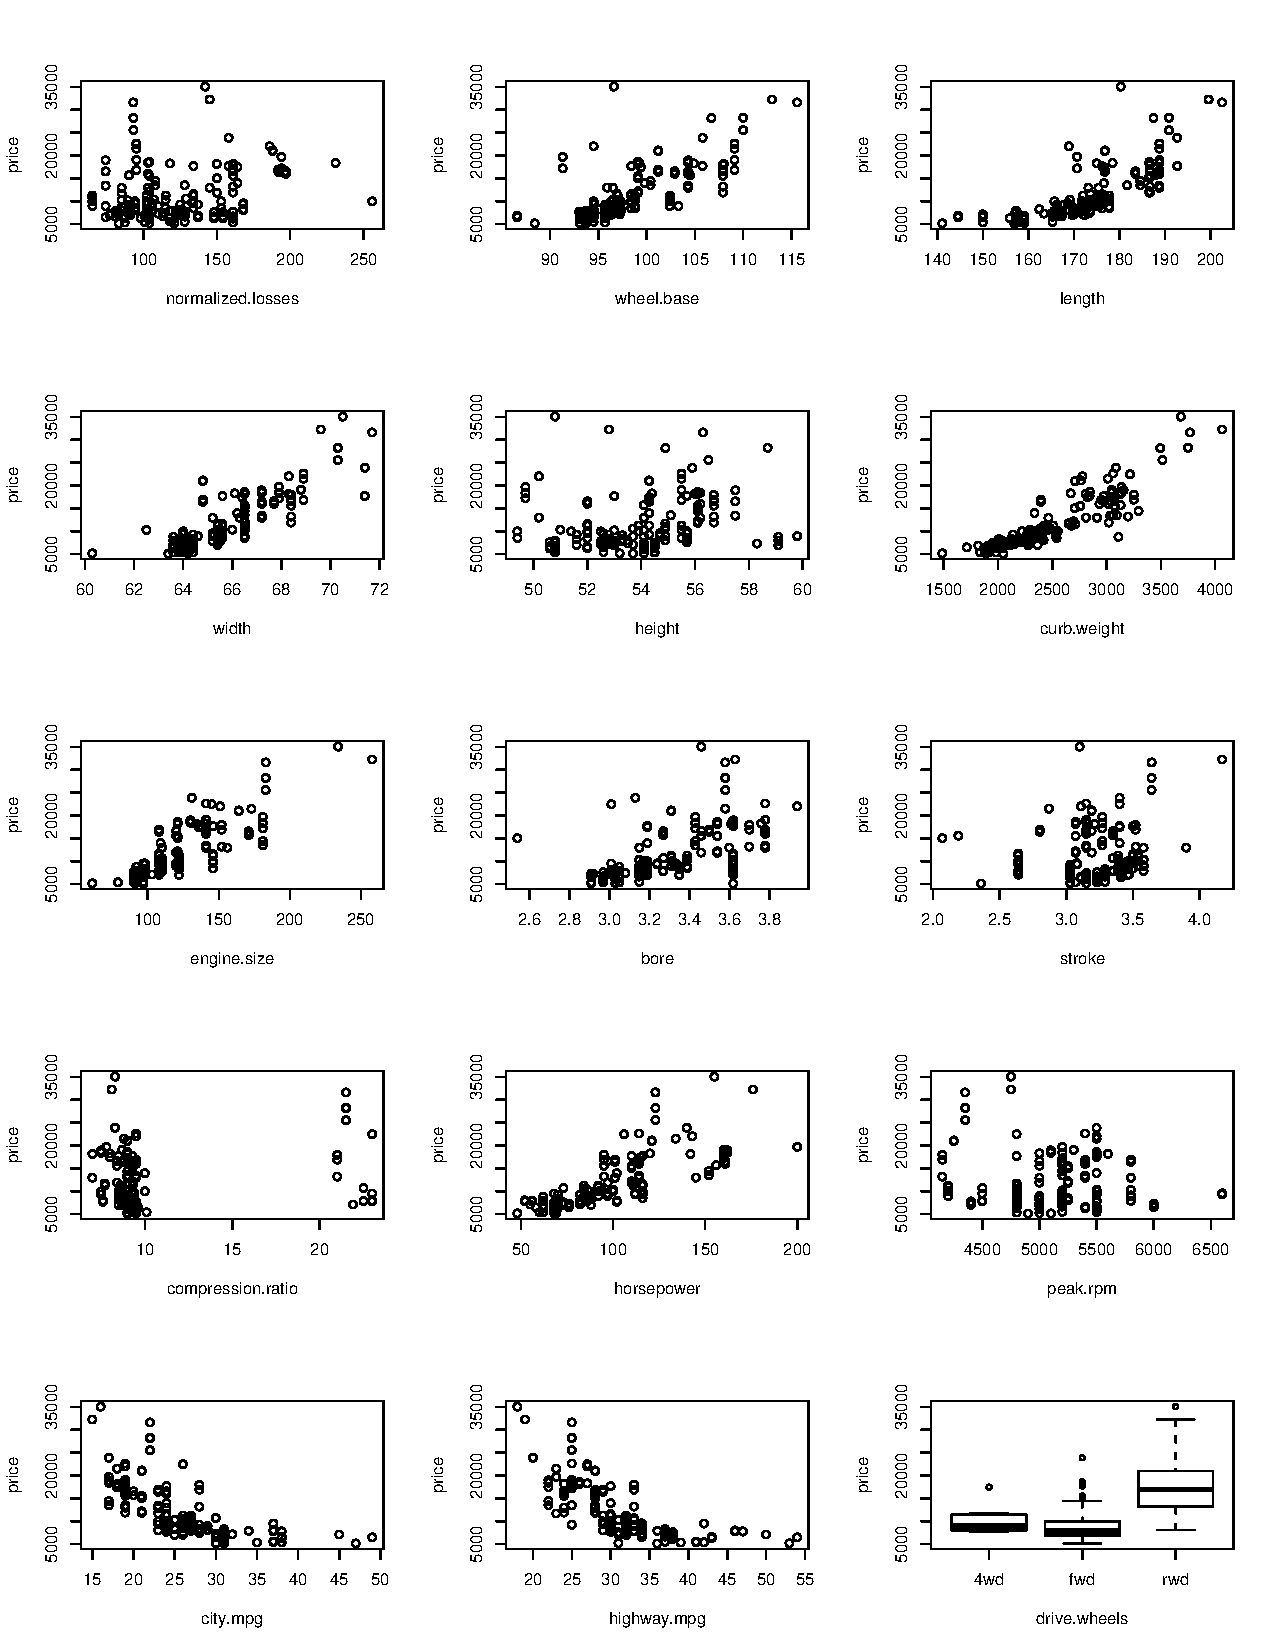
\includegraphics[width=\textwidth]{priceVsAllNum}
\caption{Response variable `price' versus regressors.}
\label{fig:priceVsAllNum}
\end{figure}

\begin{figure}[hbpt]
\centering
 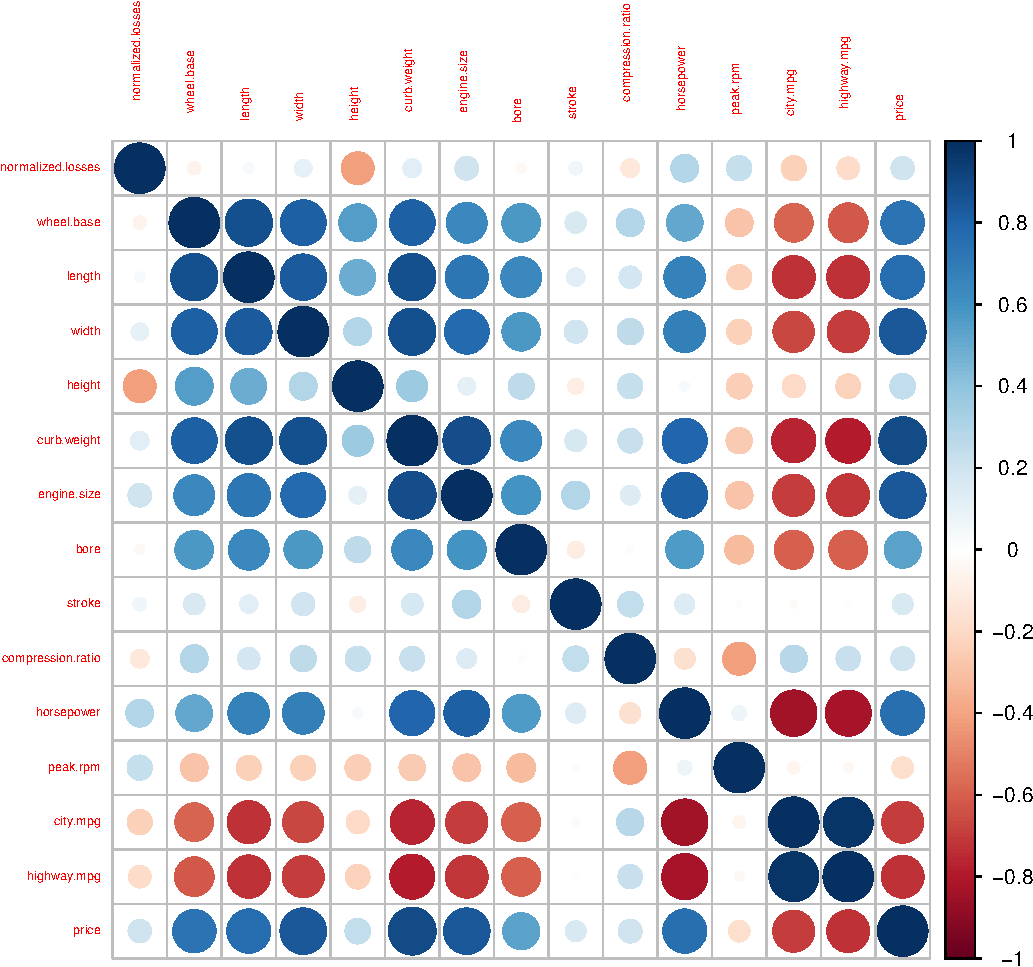
\includegraphics[width=\textwidth]{corrplot}
\caption{Correlation matrix plot.}
\label{fig:corrplot}
\end{figure}



%logarithmicTransformation
\begin{figure}[hbpt]
\centering
 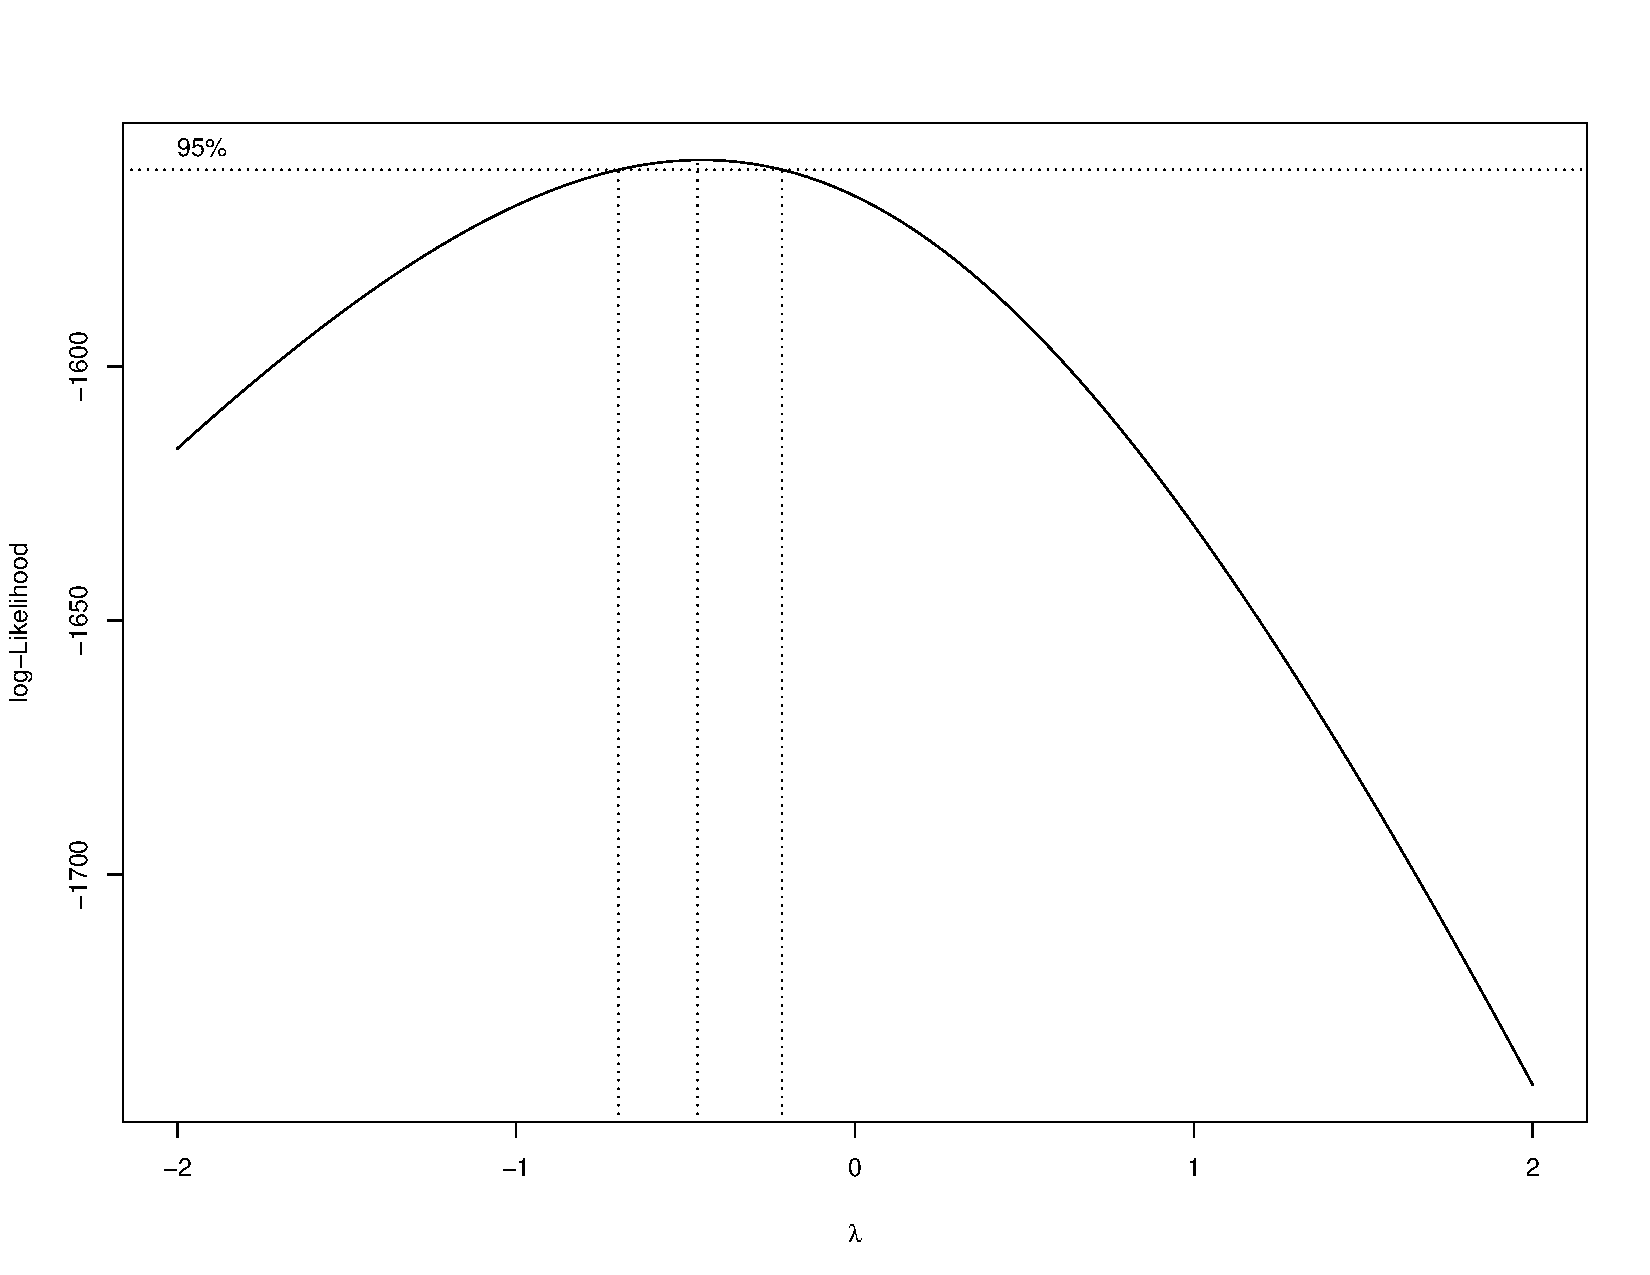
\includegraphics[width=0.65\textwidth]{boxcox}
\caption{Maximum likelihood of BoxCox transformation: $\lambda \approx -0.45$.}
\label{fig:boxcox}
\end{figure}

\begin{figure}[hbpt]
\centering
 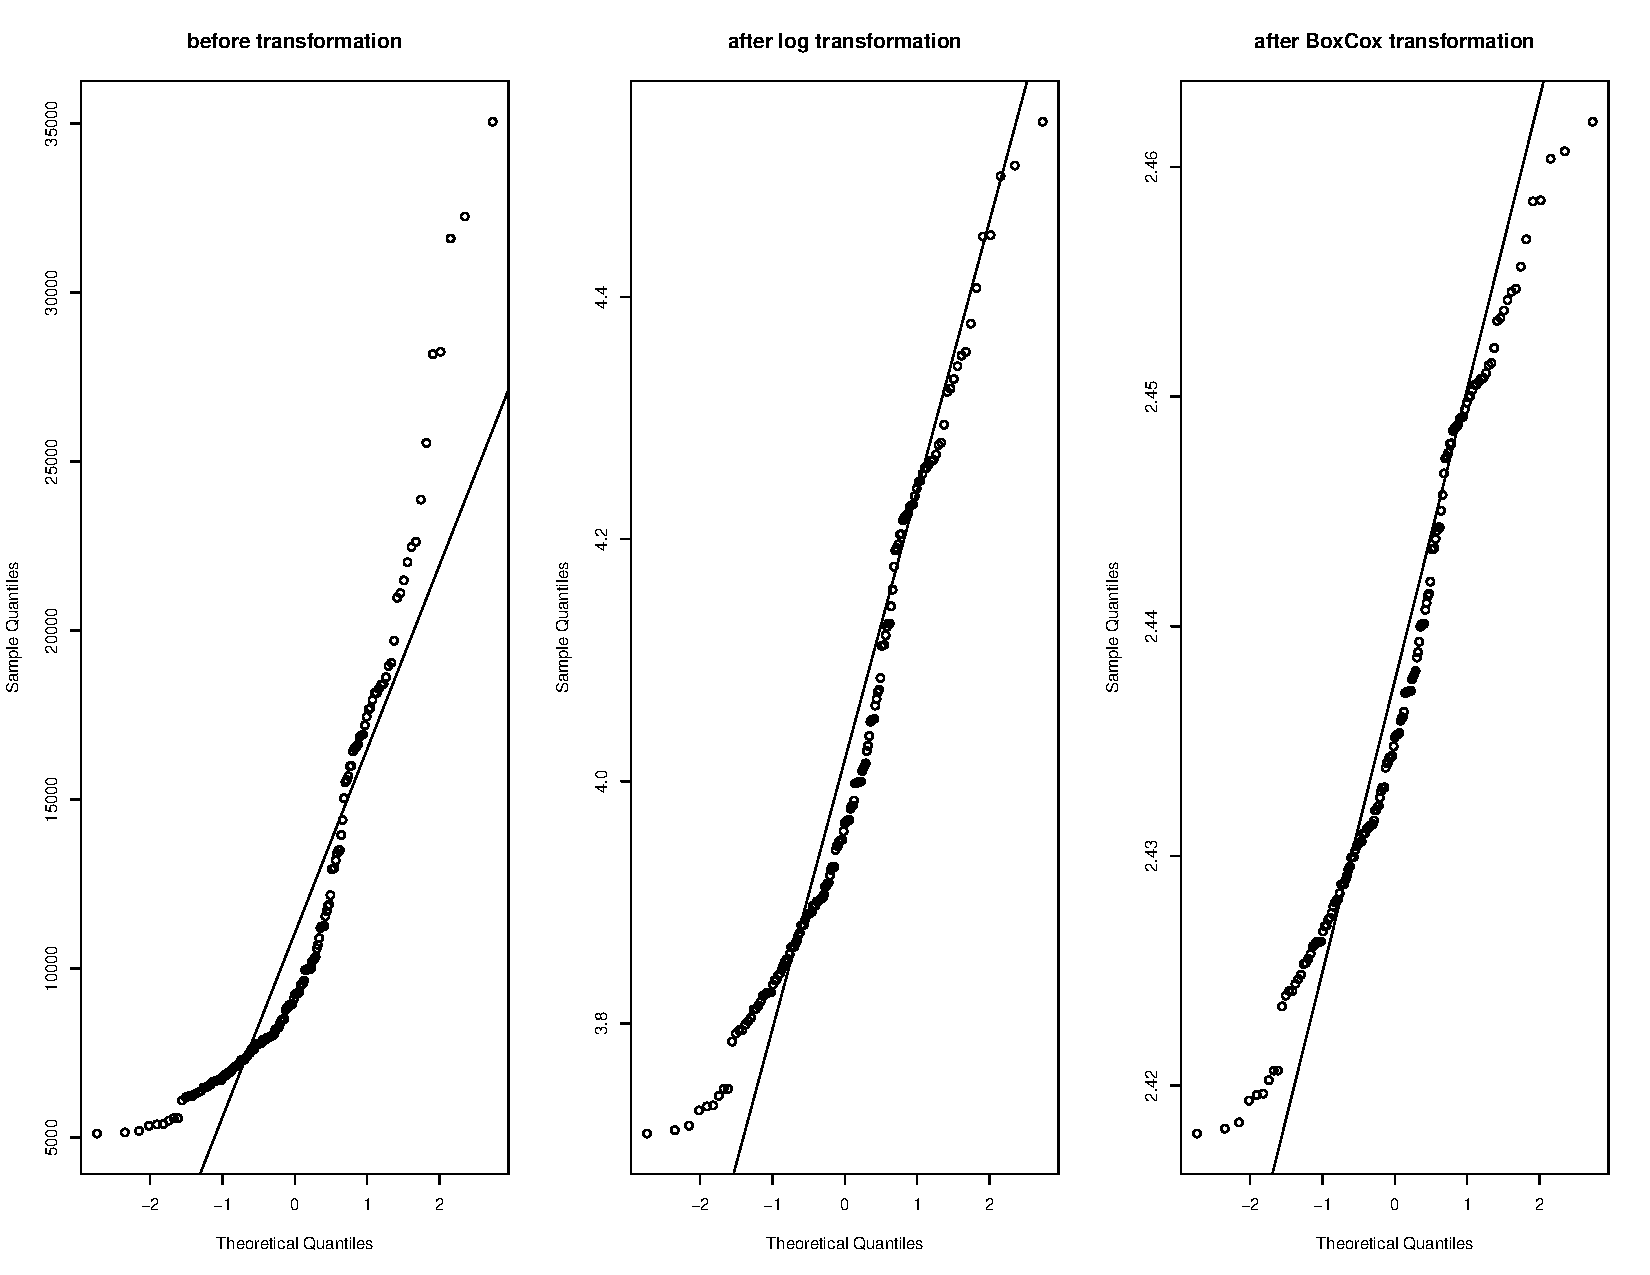
\includegraphics[width=0.85\textwidth]{logarithmicTransformation}
\caption{Transformation of the price improves normality.}
\label{fig:logarithmicTransformation}
\end{figure}

\begin{figure}[hbpt]
\centering
 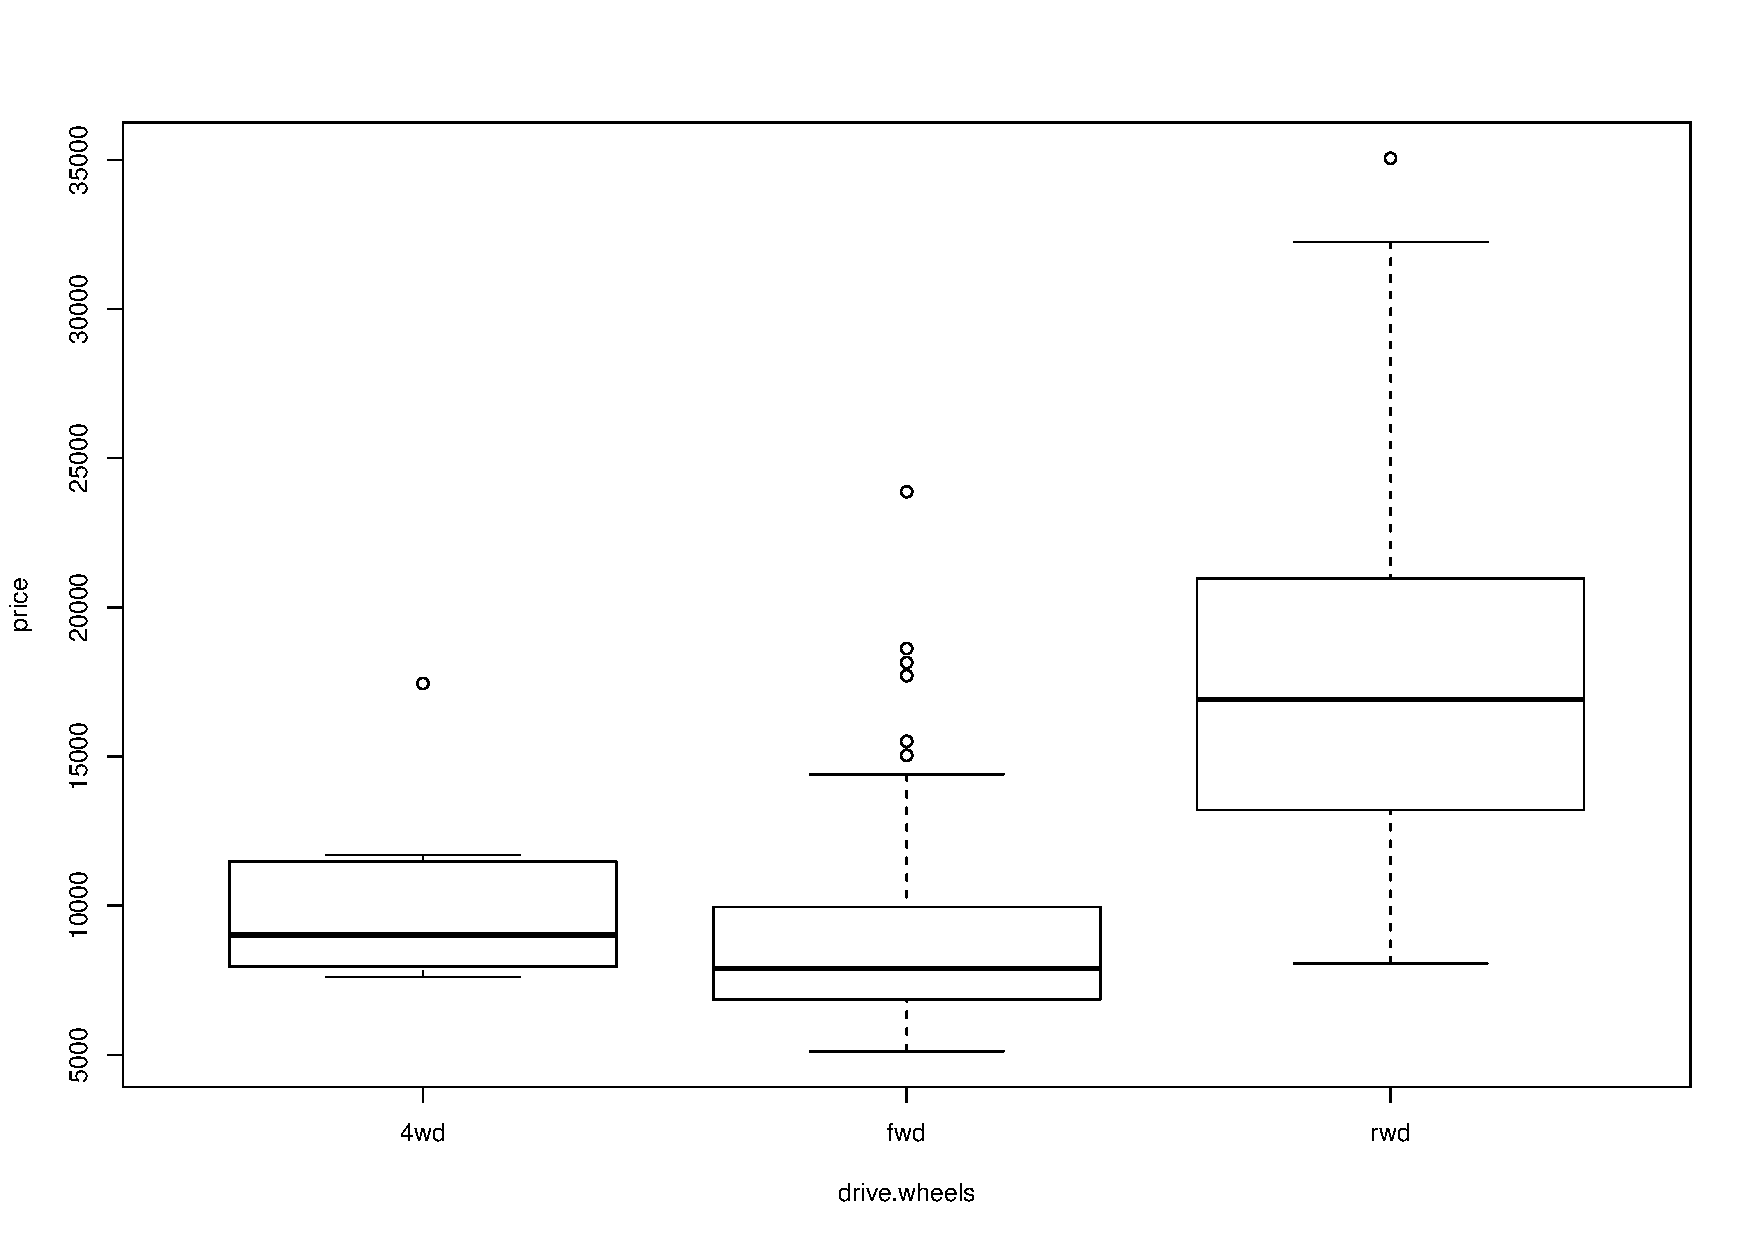
\includegraphics[width=0.95\textwidth]{boxplot_drivewheels}
\caption[Boxplot of drive-wheels versus price]{Boxplot of drive-wheels versus price---before and after BoxCox transformation.}
\label{fig:drivewheelsbox}
\end{figure}






%%PCA
\begin{figure}
  \centering
  \subfloat[Screeplot]{\label{fig:screeplot}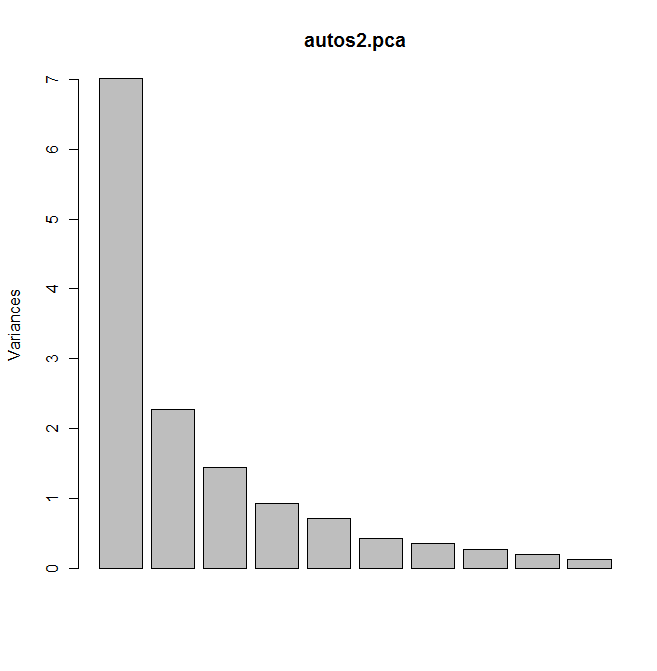
\includegraphics[width=0.5\textwidth]{pcascreeplot.png}}%screeplot}   }
  \subfloat[Biplot]{\label{fig:biplot}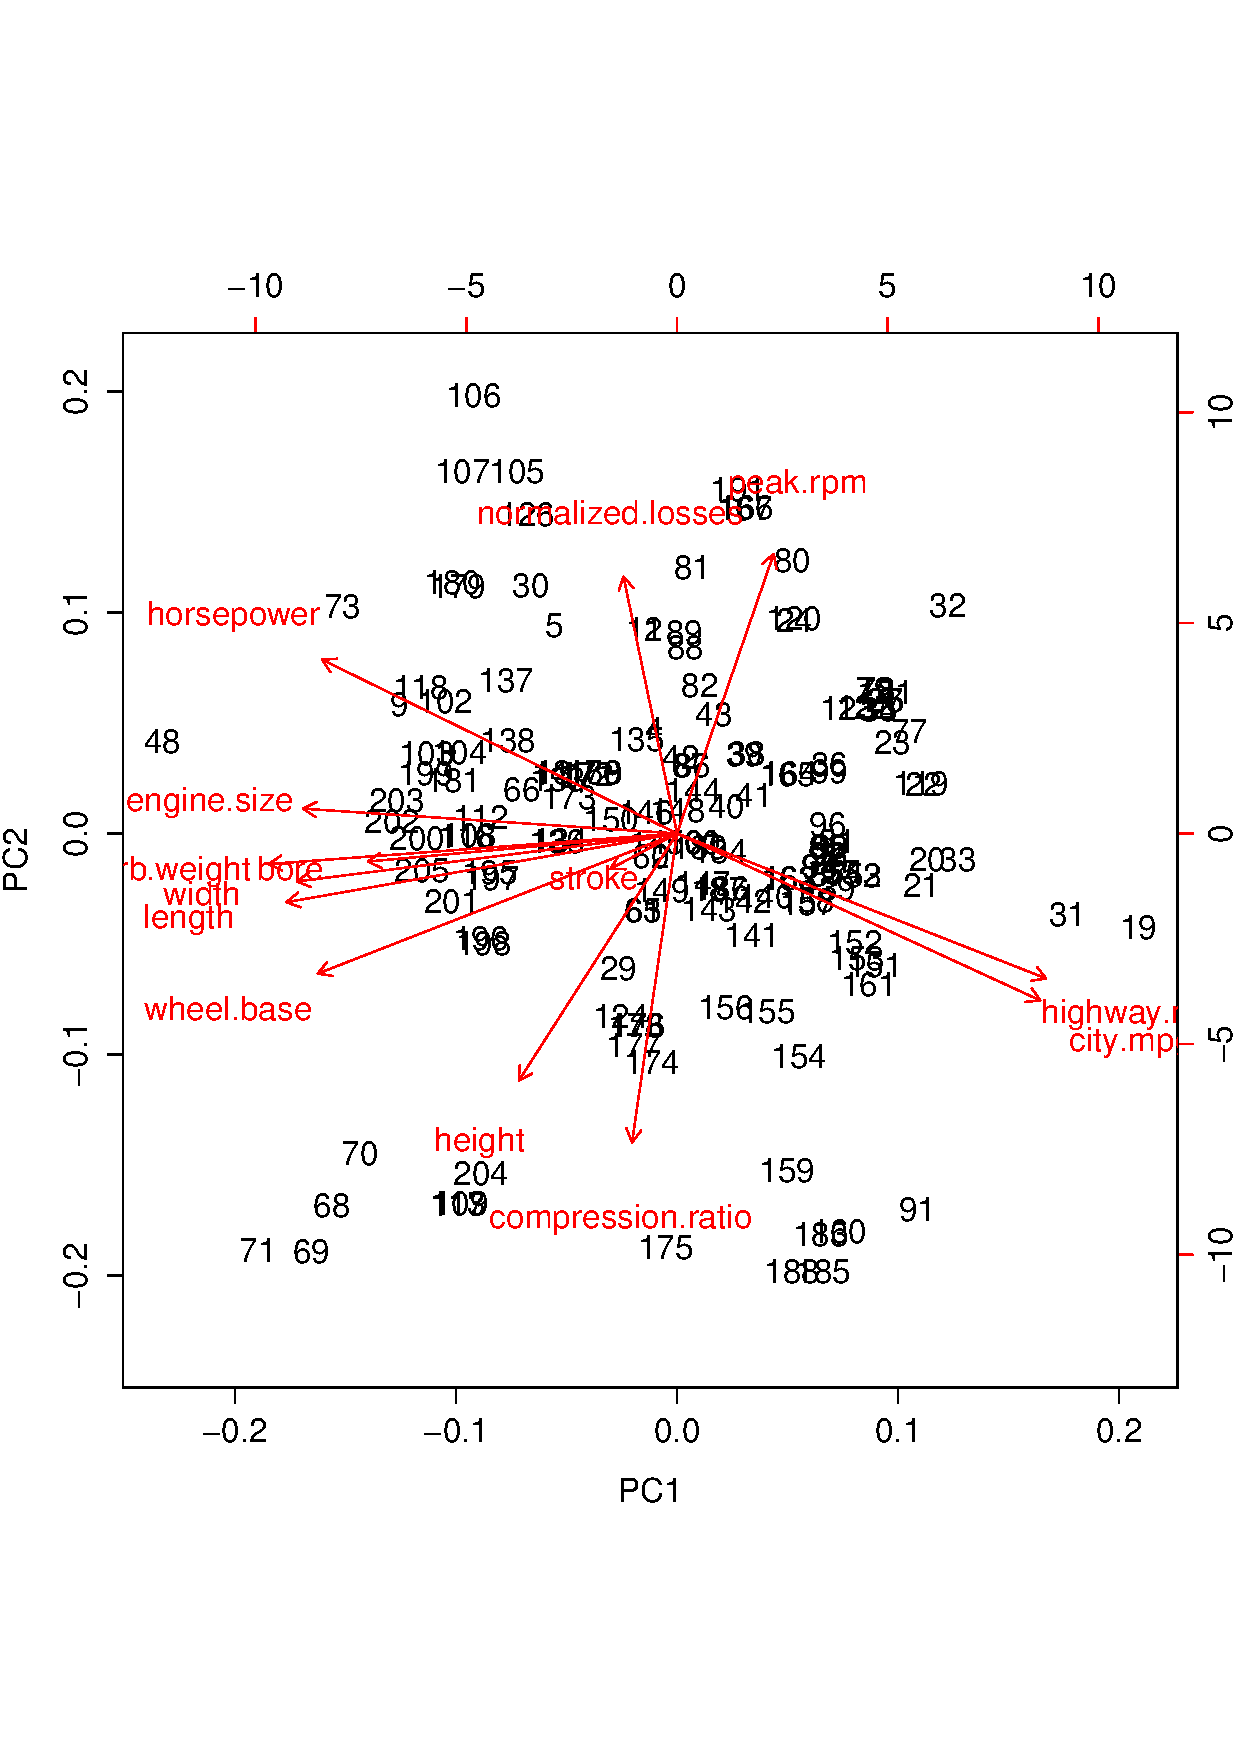
\includegraphics[width=0.5\textwidth]{biplot}}
  \caption{PCA.}
  \label{fig:pca}
\end{figure}

\begin{figure}
  \centering
  \subfloat[PCR --- normal]{\label{fig:pcrnormal}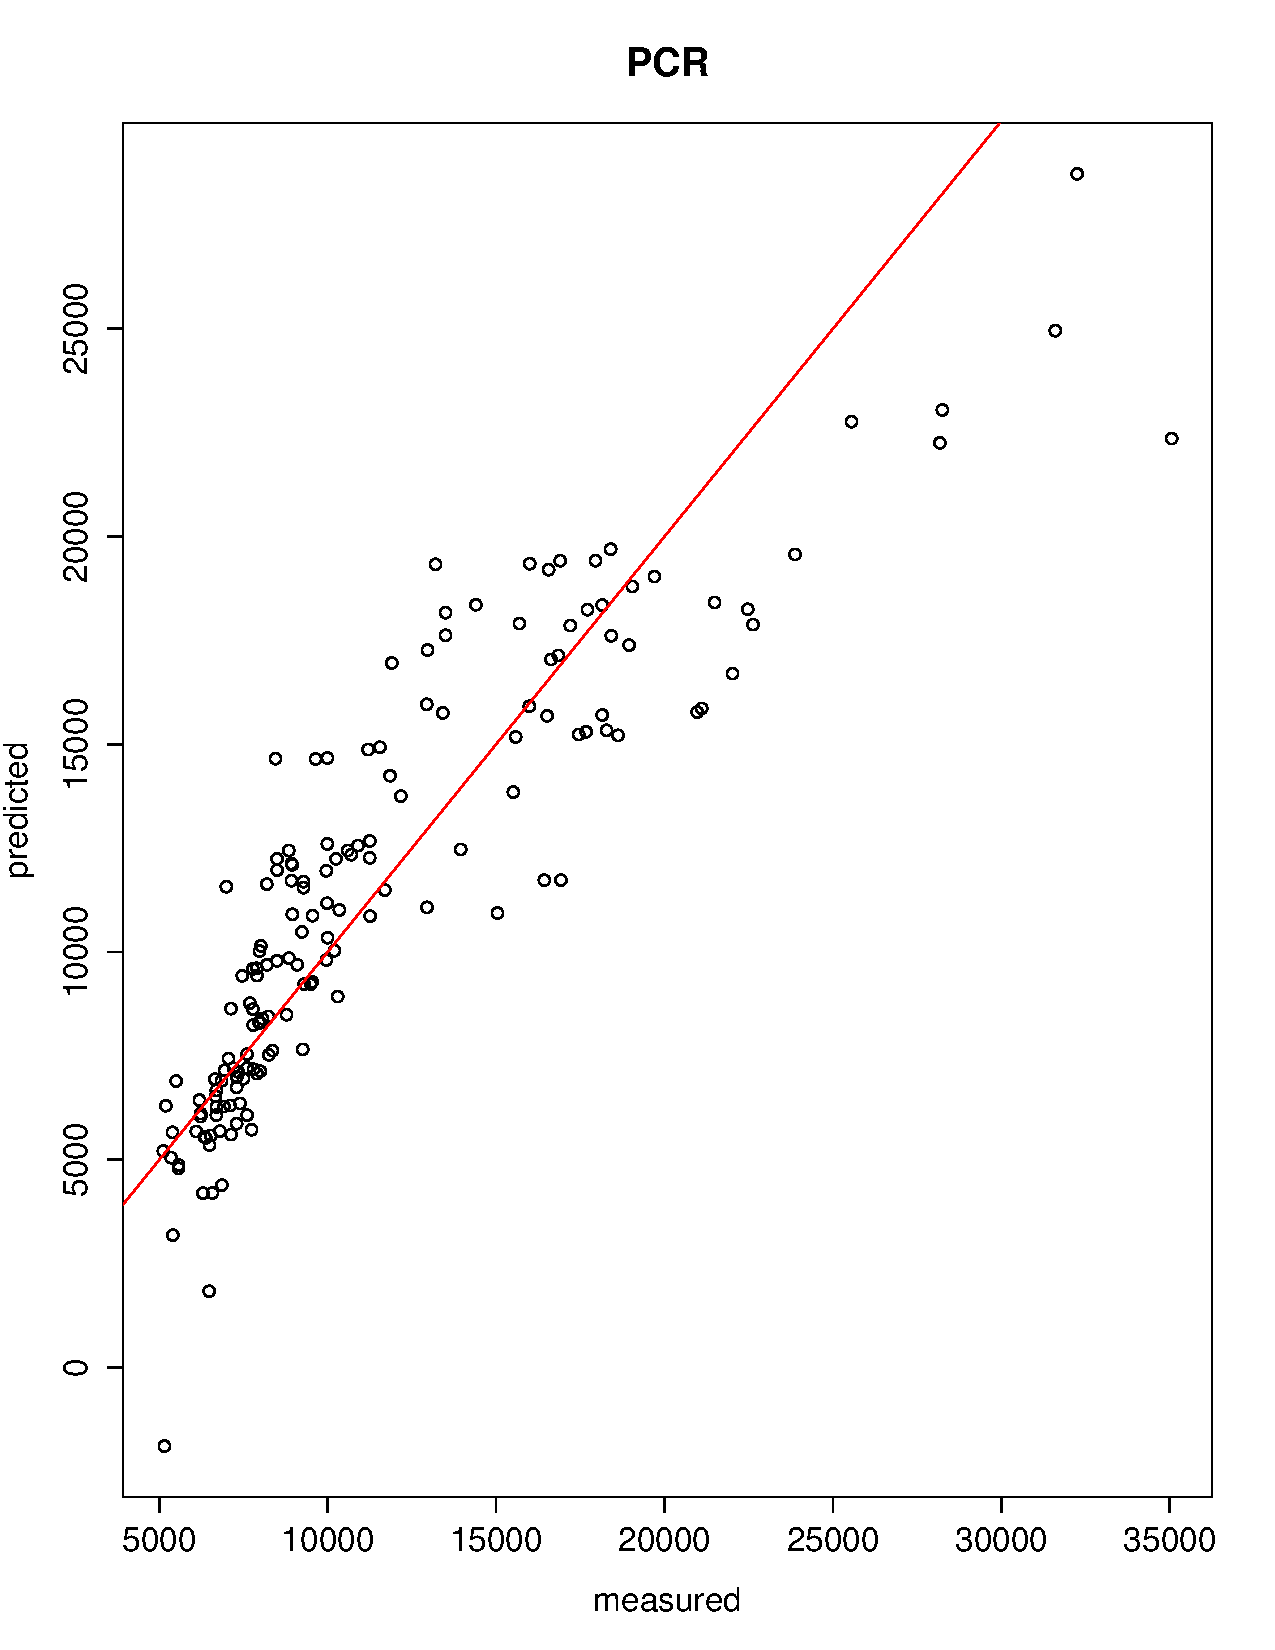
\includegraphics[width=0.5\textwidth]{PCR-pcr1.pdf}}%screeplot}   }
  \subfloat[PCR --- Box-Cox]{\label{fig:pcrbc}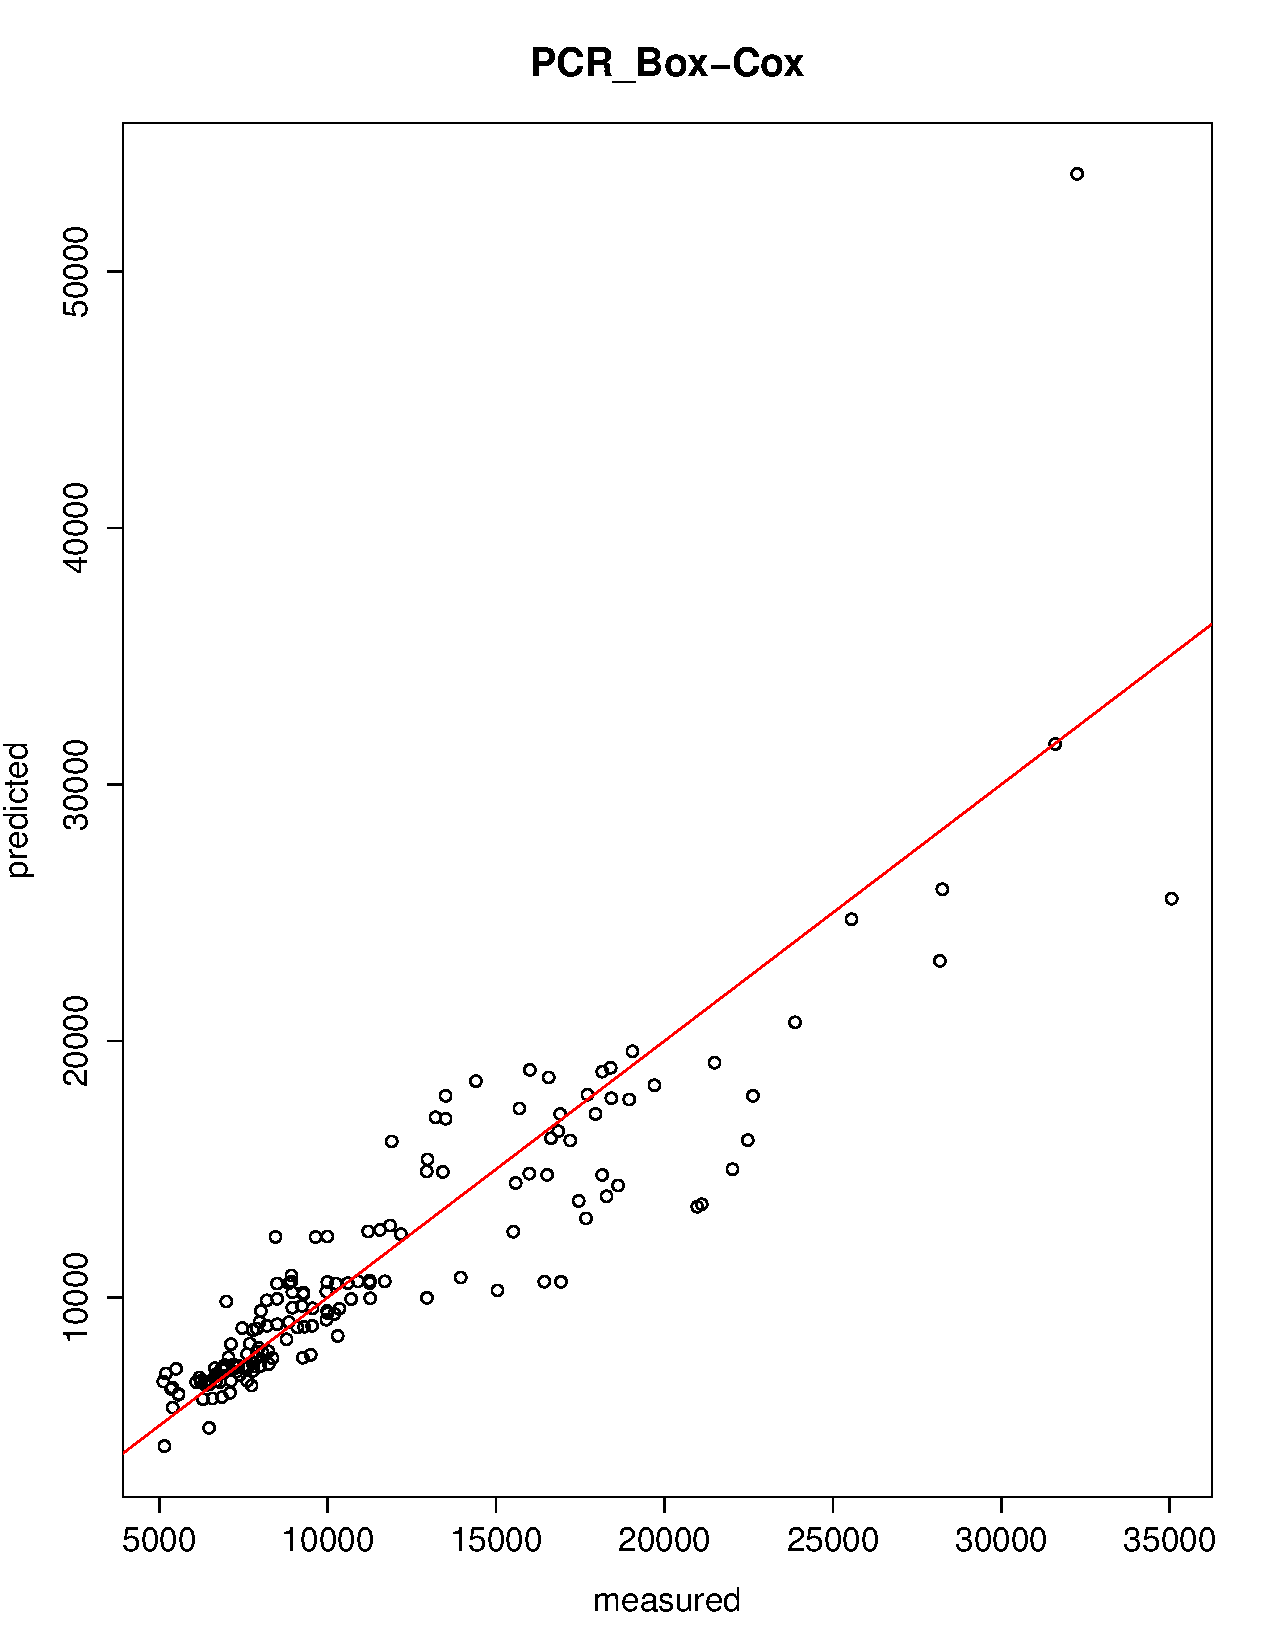
\includegraphics[width=0.5\textwidth]{PCR-boxcox.pdf}}
  \caption{PCR}
  \label{fig:pcr}
\end{figure}


\begin{figure}[hbpt]
 \centering
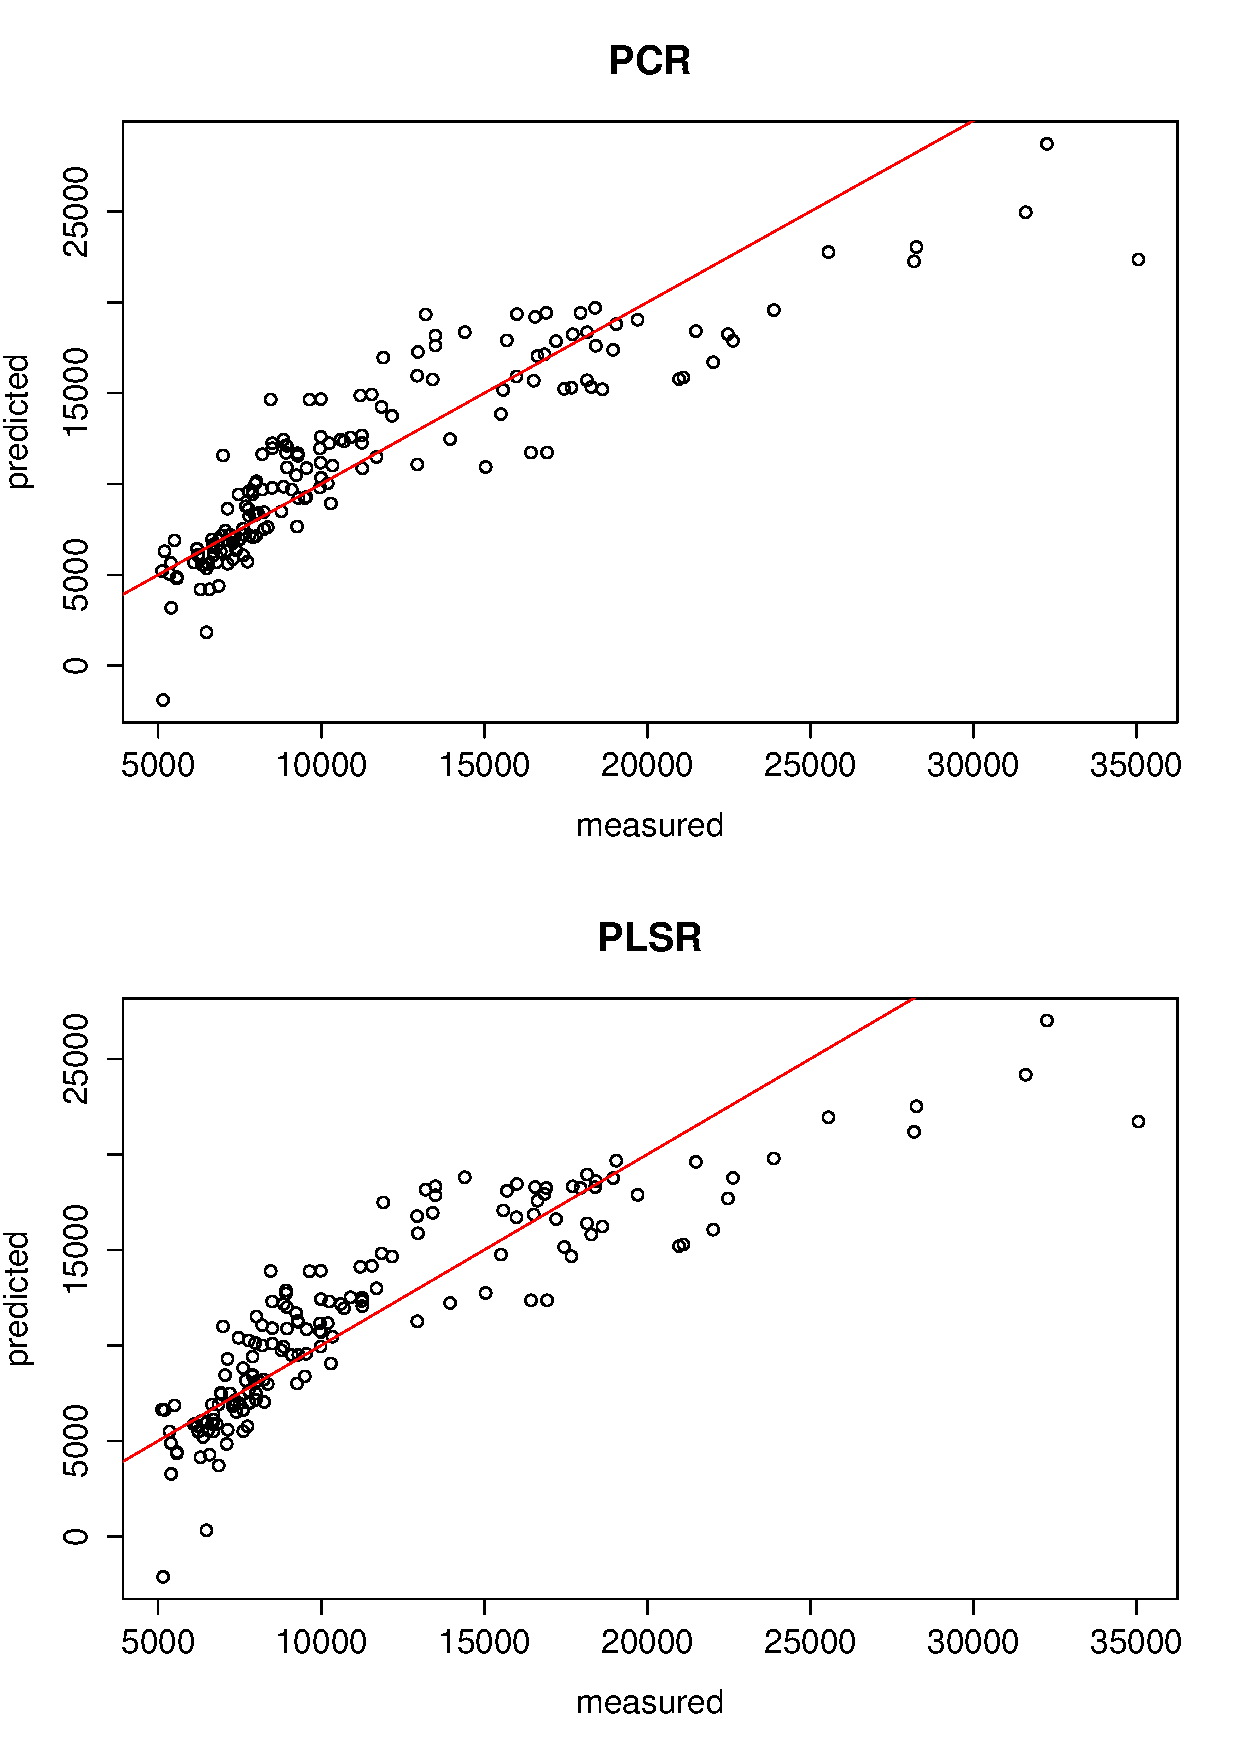
\includegraphics[width=0.95\textwidth]{PCR-PLS}%_PLS}
\caption{PCR and PLS.}
\label{fig:pcr_pls}
\end{figure}




%linear models
\begin{figure}[hbpt]
  \centering
  \subfloat[Residuals versus fitted]{\label{fig:residualsVSfitted}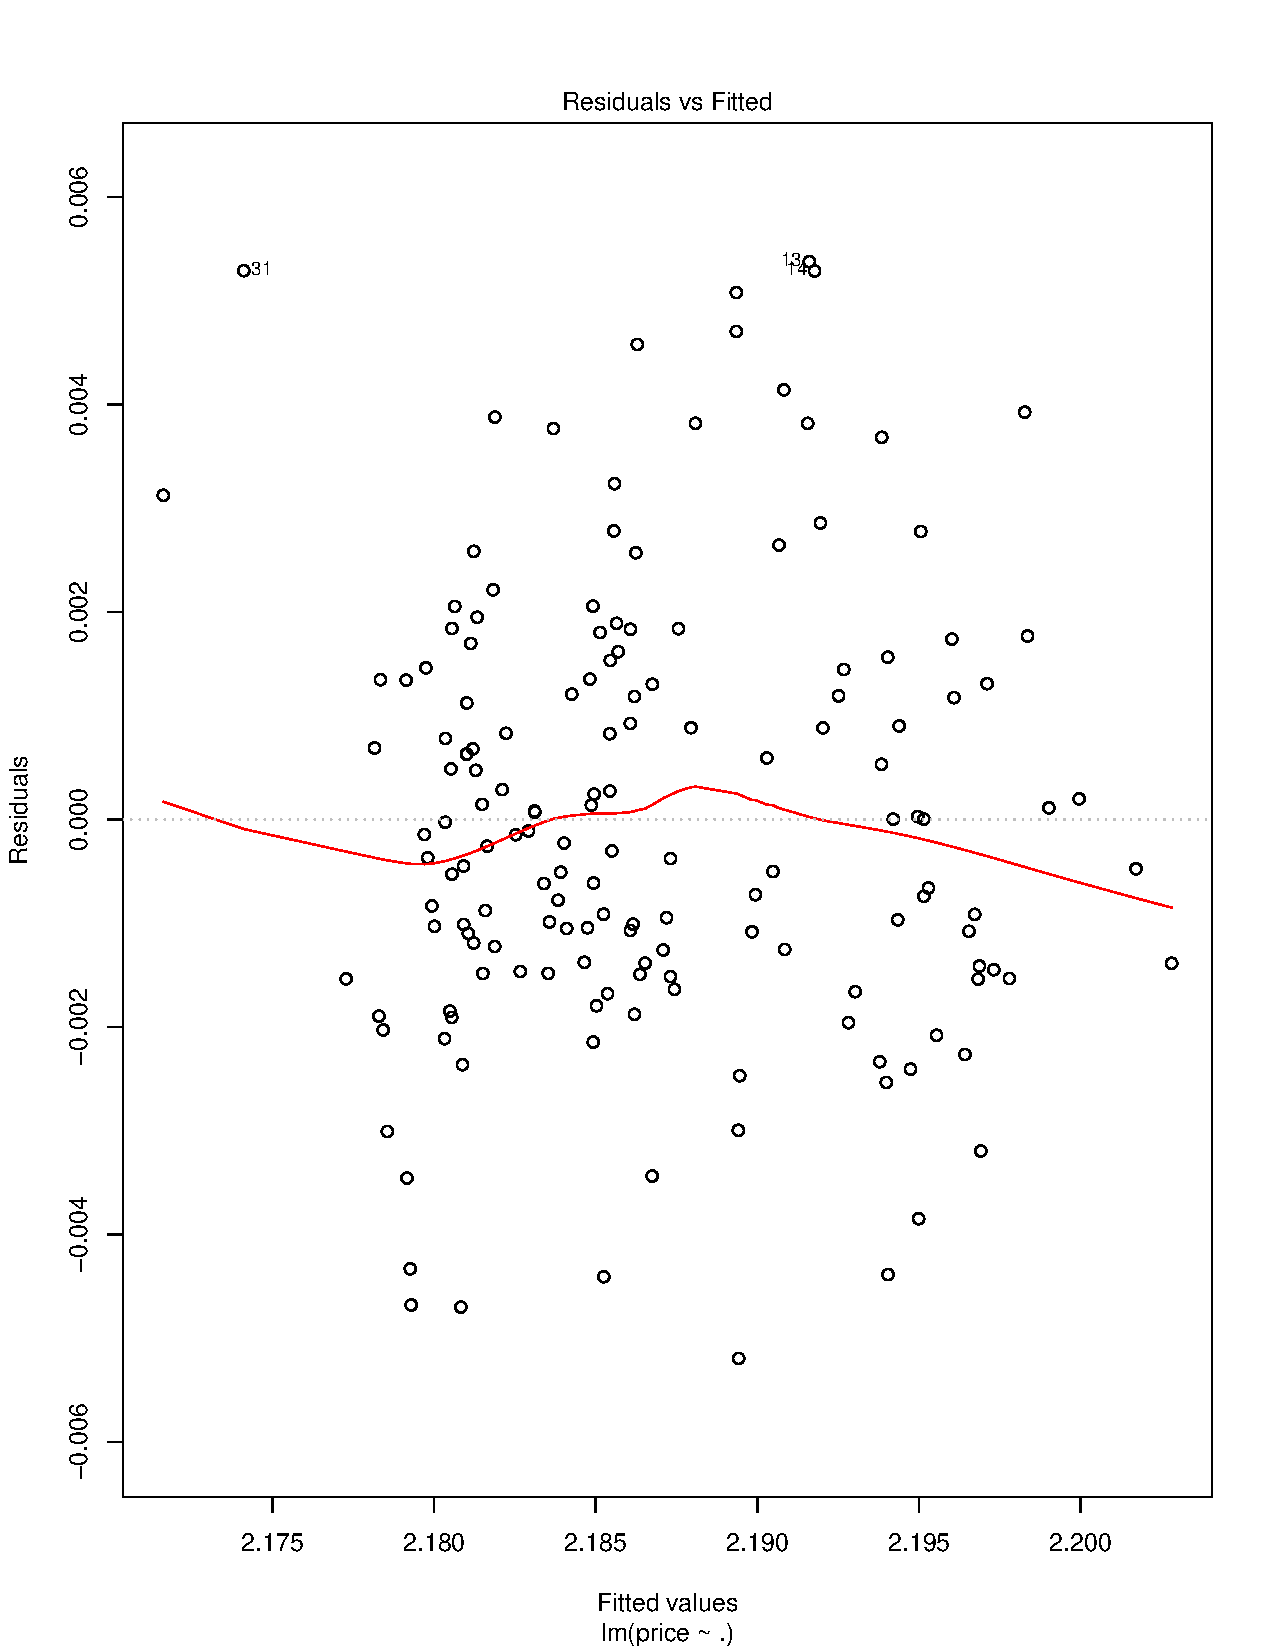
\includegraphics[width=0.5\textwidth]{residualsVSfitted}}
  \subfloat[Normal Q-Q plot of standardized residuals]{\label{fig:qqplot_residuals}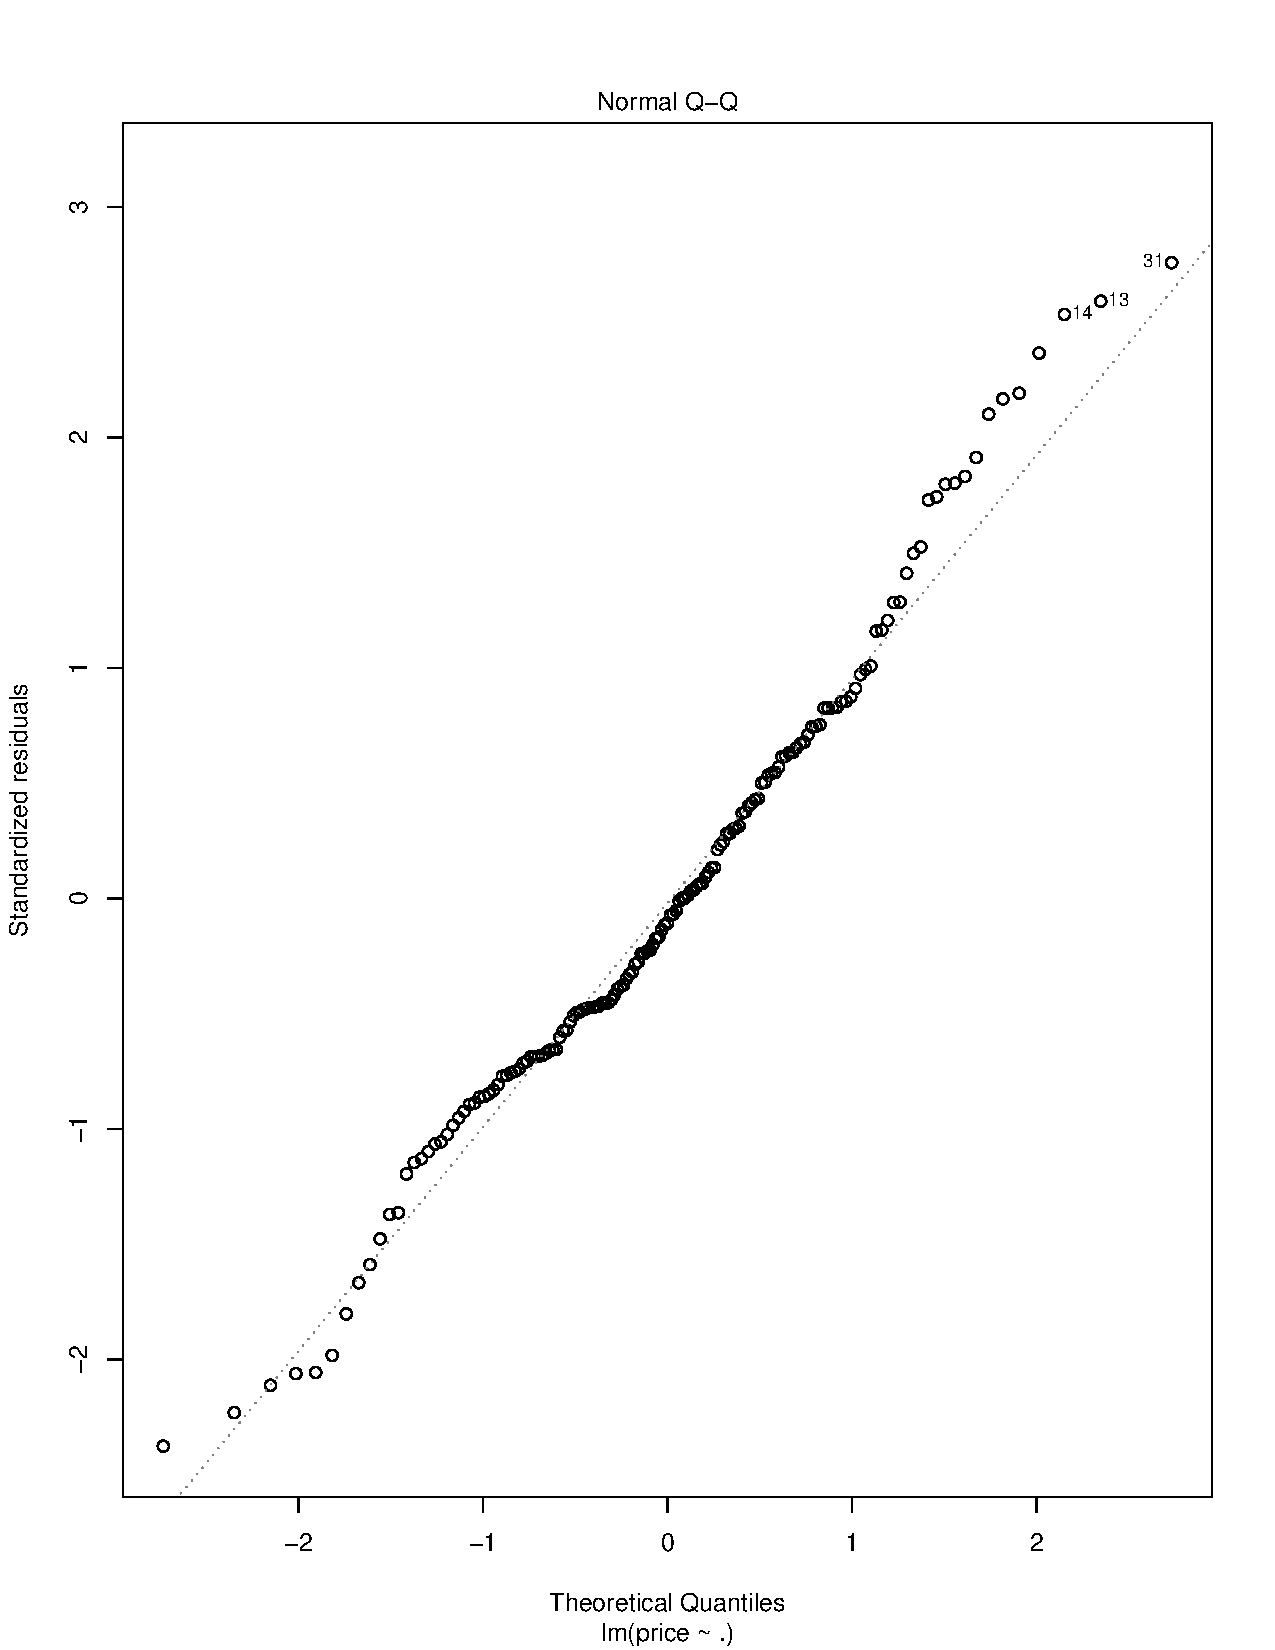
\includegraphics[width=0.5\textwidth]{qqplot_residuals}}
  \caption{Diagnostic plots for linear model using all variables as regressors.}
  \label{fig:diagnosticLM}
\end{figure}

\begin{figure}[hbpt]
  \centering
  \subfloat[Residuals versus fitted]{\label{fig:residualsVSfitted2}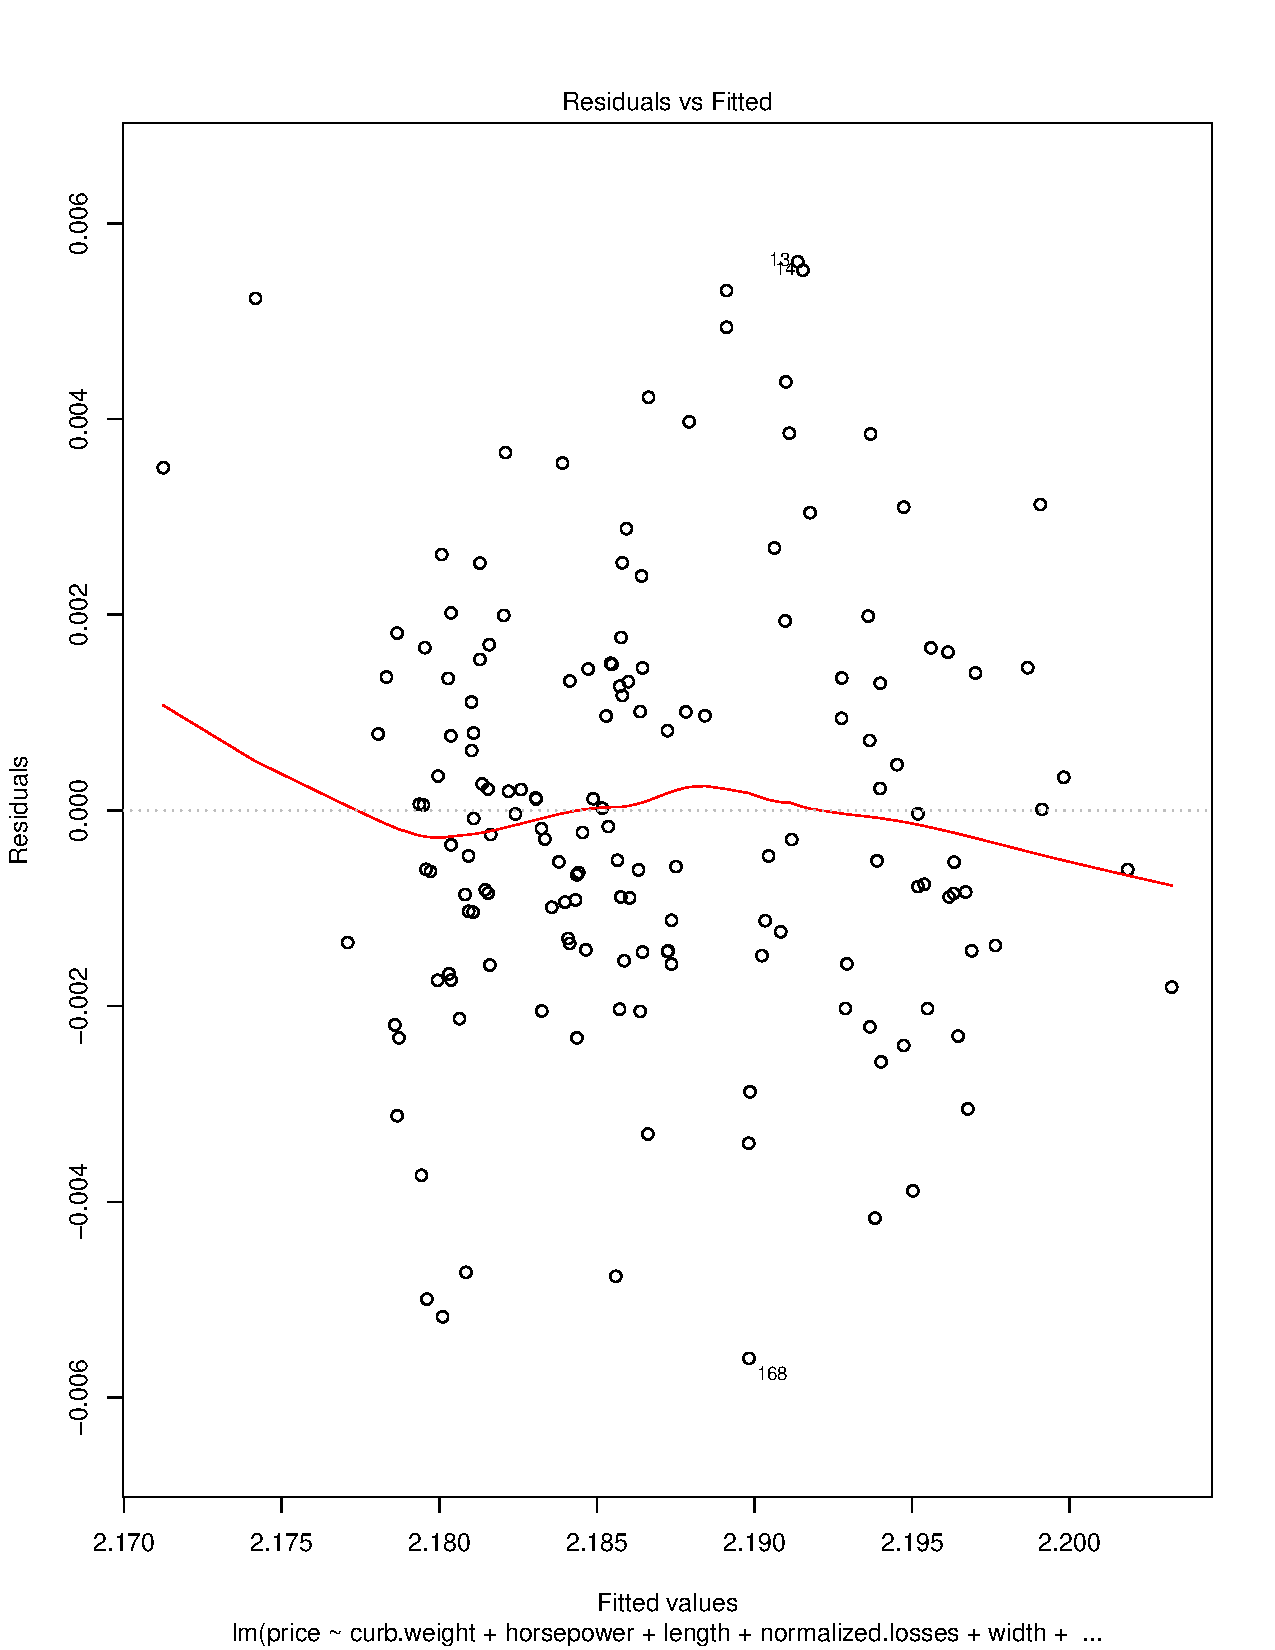
\includegraphics[width=0.5\textwidth]{residualsVSfitted2}}
  \subfloat[Normal Q-Q plot of standardized residuals]{\label{fig:qqplot_residuals2}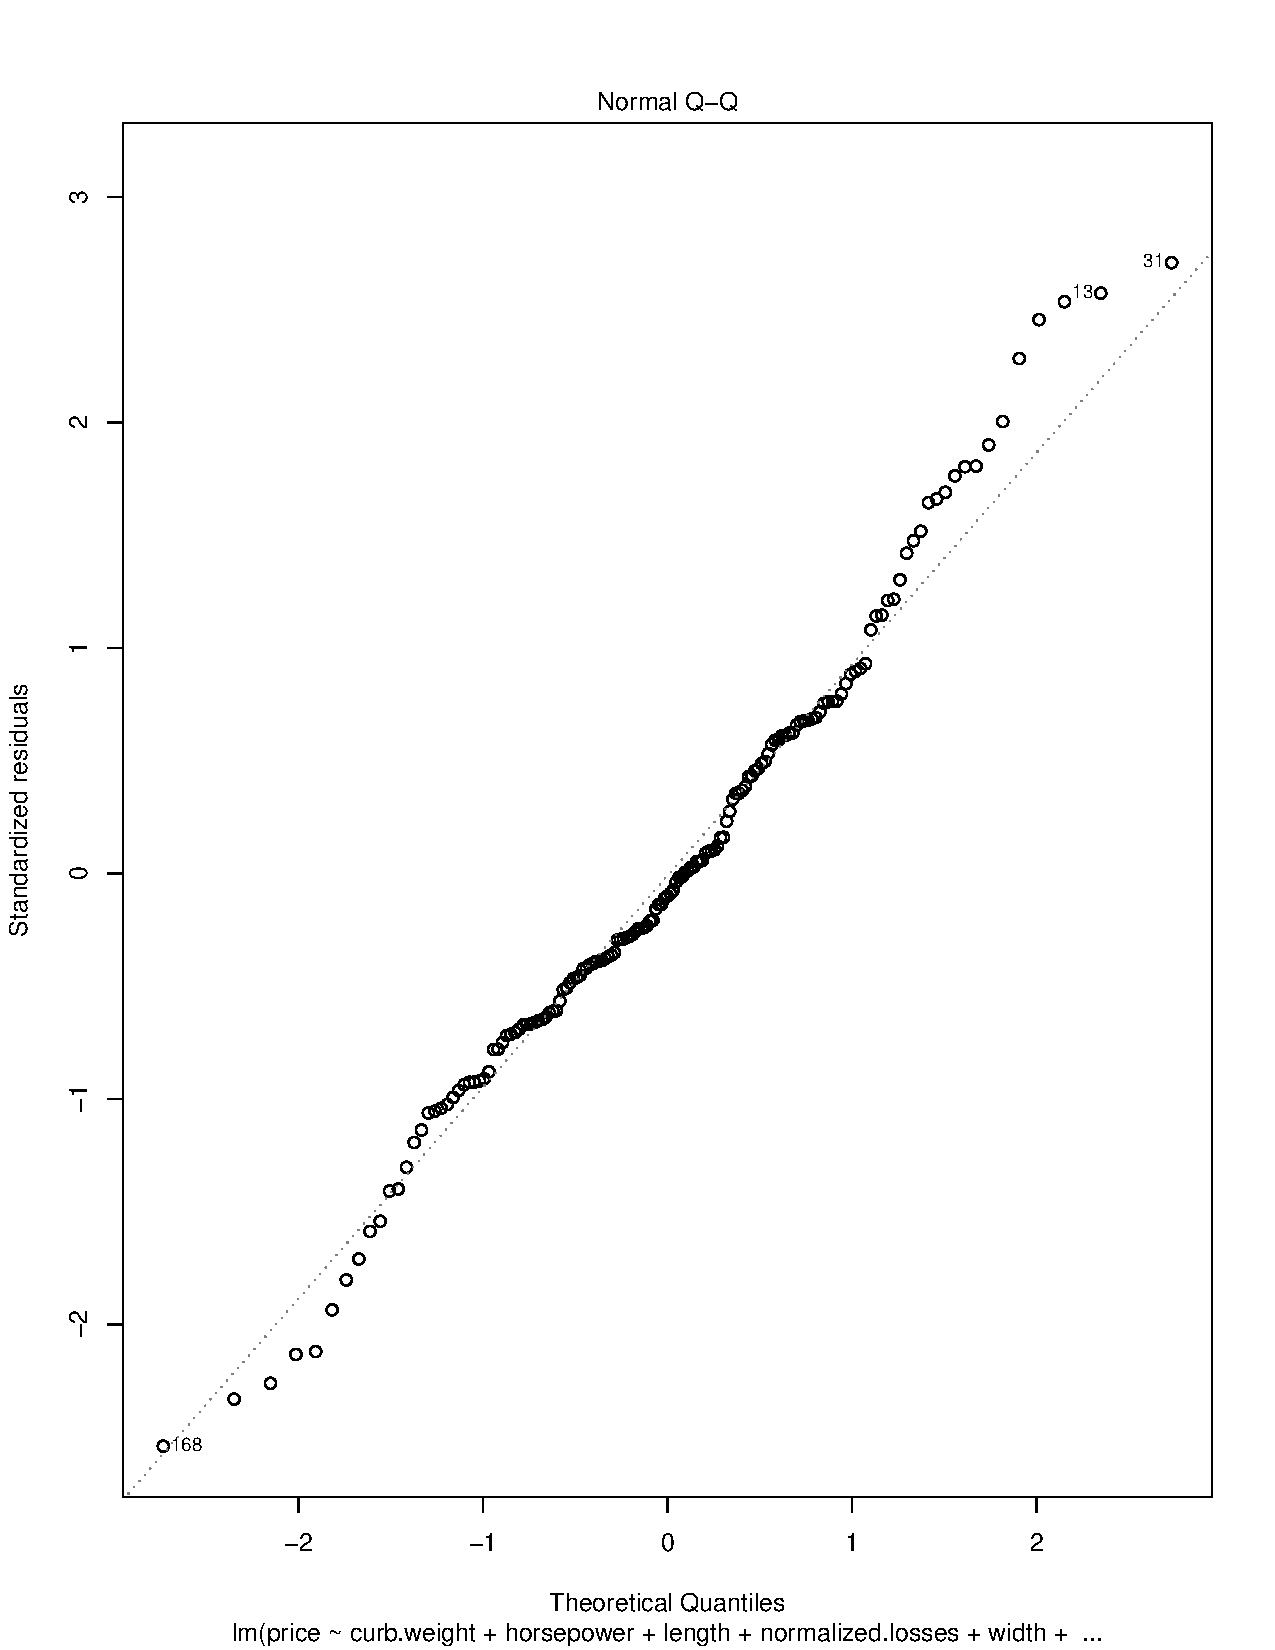
\includegraphics[width=0.5\textwidth]{qqplot_residuals2}}
  \caption{Diagnostic plots for linear model obtained by stepwise regression (AIC).}
  \label{fig:diagnosticLM2}
\end{figure}



%anova
\begin{figure}[hbpt]
 \centering
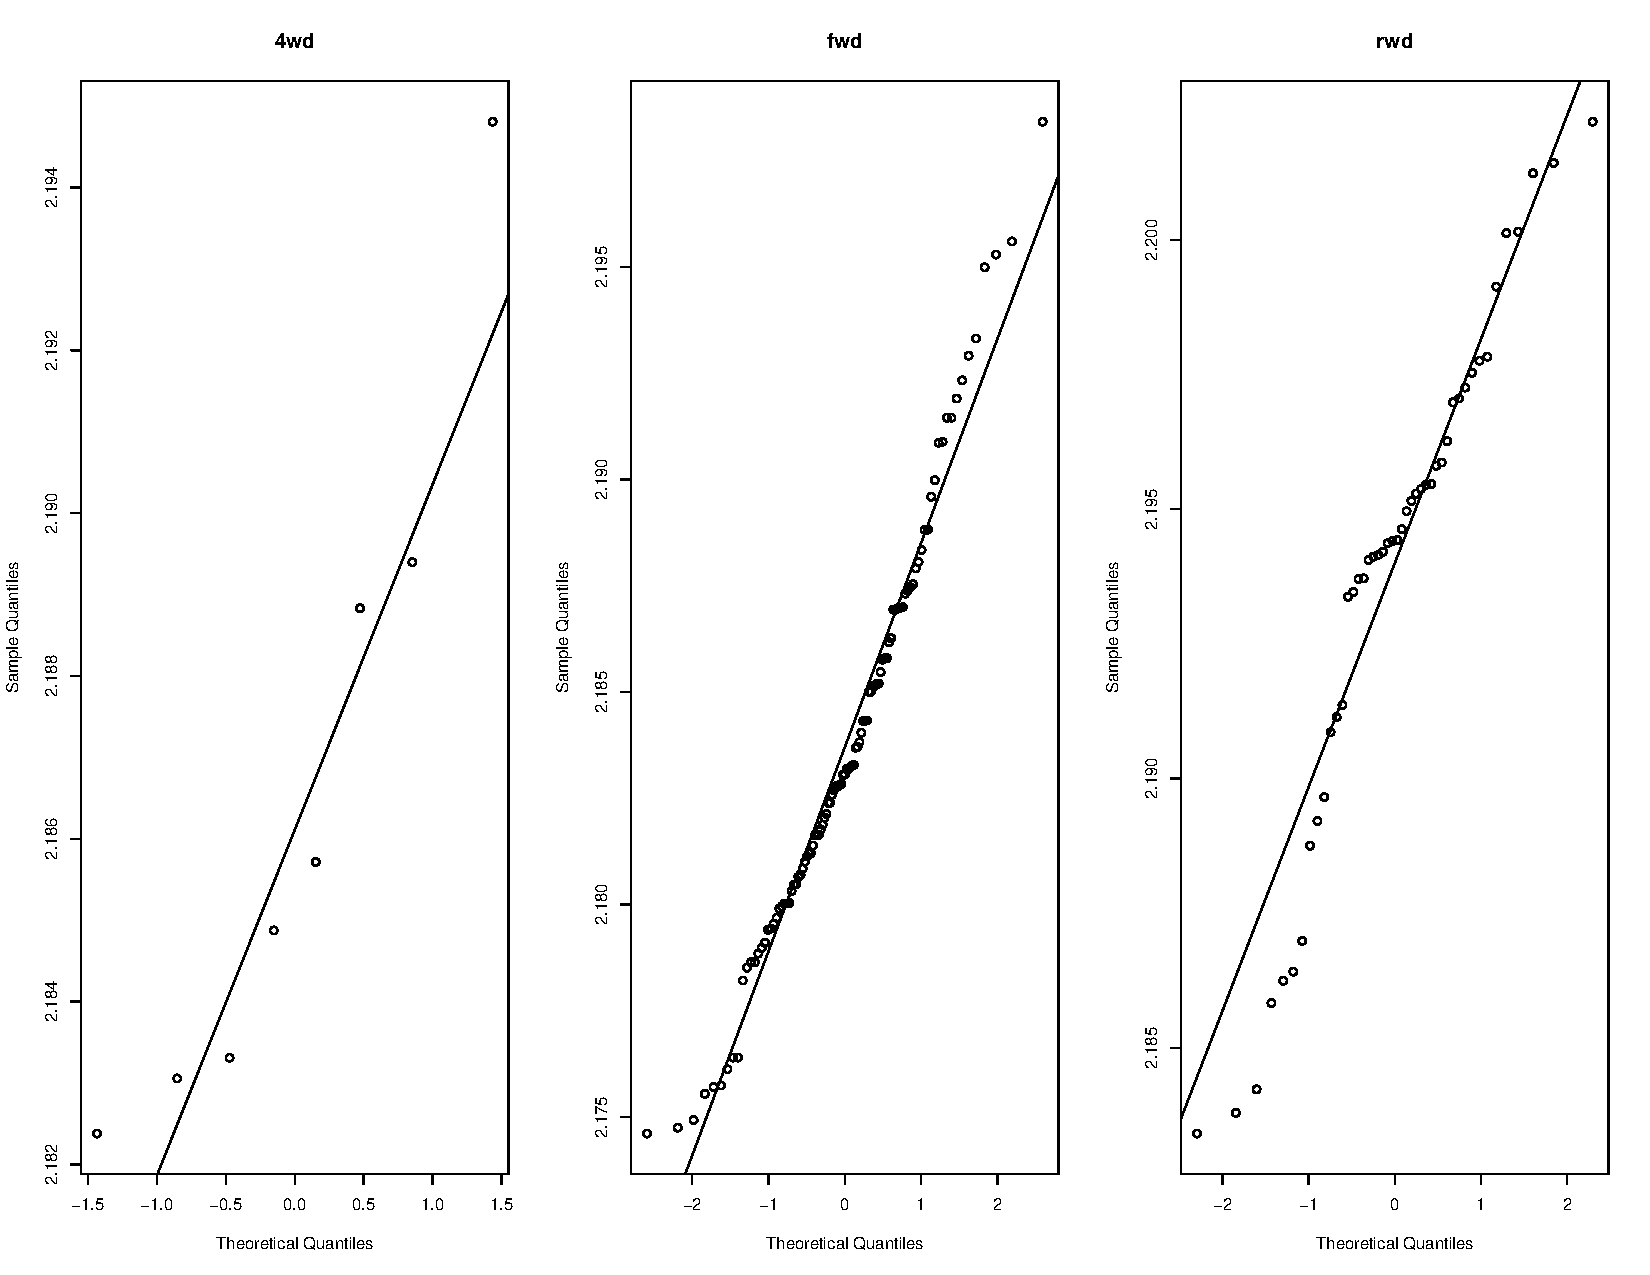
\includegraphics[width=0.95\textwidth]{normalDrivewheels.pdf}
\caption{Normal Q-Q plots of drive-wheels.}
\label{fig:qqdrive-wheel}
\end{figure}





\clearpage

\section{R-code\label{Rcode}}
Used libraries:
\begin{multicols}{2}
\begin{itemize}
 \item MASS
 \item car
 \item rggobi
 \item corrplot
 \item pls
 \item FitAR
\end{itemize}
\end{multicols}
\lstinputlisting{./R/homework2.R}
% \inputminted[]{R}{./R/homework2.R}


\clearpage
\bibliography{biblio}
\end{document} 
